%initialising document, adjust papersize, fontsize and page orientation to your needs
\documentclass[a4paper, fontsize = 8pt, landscape]{scrartcl}
\usepackage{../../../misc_files/LateX/layout_and_colours}
\makeatletter
\def\input@path{{content/summary/}{content/examples/}}
\makeatother

\title{Web-Entwicklung}
\author{Jil Zerndt, Lucien Perret}
\date{January 2025}

\createtitlepagestyle
\createmainpagestyle
\begin{document}
\begin{multicols}{3}
	\thispagestyle{TitlePageStyle}
	\maketitle
	\sffamily
	
\begin{definition}{WEB-Architektur}
    
    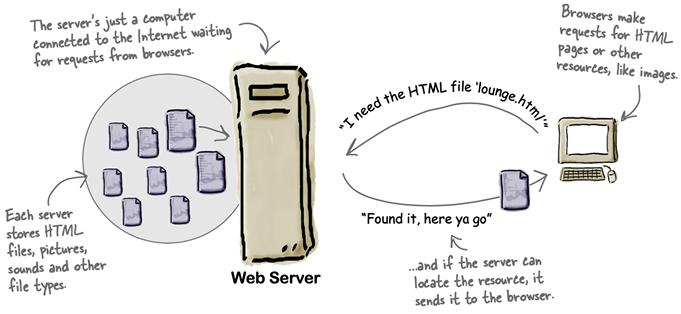
\includegraphics[width=1\linewidth]{images/web_architektur.png}
\end{definition}

\begin{concept}{Technologien}
    
    Client-Seitig $\rightarrow$ Front-end Entwickler
    \begin{itemize}
        \item Beschränkt auf das, was der Browser kann
        \item HTML + CSS + JavaScript + noch ein paar Sachen
    \end{itemize}

    Server-Seitig $\rightarrow$ Back-end Entwickler
    \begin{itemize}
        \item Praktisch unbeschränkt: Plattform, Programmiersprache, ...
        \item Erzeugt und gesendet wird das, was der Browser kann
    \end{itemize}
\end{concept}
	\raggedcolumns
	
	\section{JavaScript}

\subsection{Grundlagen und Datentypen}

\begin{concept}{JavaScript Grundlagen}
    \begin{itemize}
        \item Veröffentlicht 1995 für Netscape Navigator 2.0
        \item Entwickelt von Brendan Eich
        \item Dynamisches Typenkonzept
        \item Objektorientierter und funktionaler Stil möglich
        \item Wichtigste Programmiersprache für Webanwendungen
        \item Läuft im Browser und serverseitig (Node.js)
    \end{itemize}
\end{concept}

\begin{formula}{Web-Konsole}
    JavaScript Console im Browser und Node.js:
    \begin{itemize}
        \item \texttt{console.log(message)}: Gibt eine Nachricht aus
        \item \texttt{console.clear()}: Löscht die Konsole
        \item \texttt{console.trace(message)}: Stack trace ausgeben
        \item \texttt{console.error(message)}: stderr ausgeben
        \item \texttt{console.time()}: Timer starten
        \item \texttt{console.timeEnd()}: Timer stoppen
    \end{itemize}
\end{formula}

\begin{definition}{Datentypen}
    Primitive Datentypen:
    \begin{itemize}
        \item \texttt{number}: 64-Bit Floating Point (IEEE 754)
            \begin{itemize}
                \item \texttt{Infinity}: $1/0$
                \item \texttt{NaN}: Not a Number ($0/0$)
            \end{itemize}
        \item \texttt{bigint}: Ganzzahlen beliebiger Größe (mit n am Ende)
        \item \texttt{string}: Zeichenketten in \texttt{''}, \texttt{""} oder \texttt{``}
        \item \texttt{boolean}: \texttt{true} oder \texttt{false}
        \item \texttt{undefined}: Variable deklariert aber nicht initialisiert
        \item \texttt{null}: Variable bewusst ohne Wert
        \item \texttt{symbol}: Eindeutiger Identifier
    \end{itemize}
\end{definition}

\begin{KR}{typeof-Operator}
\begin{lstlisting}[language=JavaScript, style=basesmol]
typeof 42          // 'number'
typeof 42n         // 'bigint'
typeof "text"      // 'string'
typeof true        // 'boolean'
typeof undefined   // 'undefined'
typeof null        // 'object' (!)
typeof {}          // 'object'
typeof []          // 'object'
typeof (() => {})  // 'function'
typeof Infinity    // 'number'
typeof NaN         // 'number'
typeof 'number'    // 'string'
\end{lstlisting}
\end{KR}

\begin{theorem}{Variablenbindung}\\
    JavaScript kennt drei Arten der Variablendeklaration:
    \begin{itemize}
        \item \texttt{var}
            \begin{itemize}
                \item Scope: Funktions-Scope
                \item Kann neu deklariert werden
                \item Wird gehoistet
            \end{itemize}
        \item \texttt{let}
            \begin{itemize}
                \item Scope: Block-Scope
                \item Moderne Variante für veränderliche Werte
                \item Keine Neudeklaration im gleichen Scope
            \end{itemize}
        \item \texttt{const}
            \begin{itemize}
                \item Scope: Block-Scope
                \item Wert kann nicht neu zugewiesen werden
                \item Referenz ist konstant (Objekte können modifiziert werden)
            \end{itemize}
    \end{itemize}
\end{theorem}

\begin{corollary}{Operatoren}
    \begin{itemize}
        \item Arithmetische Operatoren: $+, -, *, /, \%, ++, --$
        \item Zuweisungsoperatoren: $=, +=, -=, *=, /=, \%=, **=, $\\$<<=, >>=, >>>=, \&=, ^=, |=$
        \item Vergleichsoperatoren: $==, ===, !=, !==, >, <, >=, <=$
        \item Logische Operatoren: $\&\&, ||, !$
        \item Bitweise Operatoren: $\&, |, ^, ~, <<, >>, >>>$
        \item Sonstige Operatoren: \texttt{typeof}, \texttt{instanceof}
    \end{itemize}
\end{corollary}

\begin{formula}{Vergleichsoperatoren}\\
    JavaScript unterscheidet zwei Arten von Gleichheit:
    \begin{itemize}
        \item \texttt{==} und \texttt{!=}: Mit Typumwandlung
        \item \texttt{===} und \texttt{!==}: Ohne Typumwandlung (strikt)
    \end{itemize}
\begin{lstlisting}[language=JavaScript, style=basesmol]
5 == "5"     // true  (Typumwandlung)
5 === "5"    // false (keine Typumwandlung)
null == undefined    // true
null === undefined   // false
\end{lstlisting}
\end{formula}

\begin{KR}{Verzweigungen\text{,} Wiederholung und Switch Case}
    \begin{itemize}
        \item \texttt{if (condition) \{...\} else \{...\}}
        \item \texttt{switch (expression) \{ case x: ... break; default: ... \}}
        \item \texttt{for (initialization; condition; increment) \{...\}}
        \item \texttt{while (condition) \{...\}}
        \item \texttt{do \{...\} while (condition)}
        \item \texttt{for (let x of iterable) \{...\}}
    \end{itemize}
\end{KR}

\begin{examplecode}{Kontrollstrukturen}
\begin{lstlisting}[language=JavaScript, style=basesmol]
// If-Statement
if (condition) {
    // code
} else if (otherCondition) {
    // code
} else {
    // code
}

// Switch Statement
switch(value) {
    case 1:
        // code
        break;
    default:
        // code
}

// Loops
for (let i = 0; i < n; i++) { /* code */ }

while (condition) { /* code */ }

do { /* code */ } while (condition);

for (let item of array) { 
    doSomething(item);
}

for (let key in object) { 
    doSomething(object[key]);
}
\end{lstlisting}
\end{examplecode}

\subsubsection{Strings und reguläre Ausdrücke}

\begin{definition}{Strings}
    Strings in JavaScript sind:
    \begin{itemize}
        \item Sequenz von 16-Bit-Unicode-Zeichen
        \item Kein spezieller char-Typ vorhanden
        \item Definition mit einfachen ('...') oder doppelten ("...") Anführungszeichen möglich
        \item Escape-Sequenzen mit \textbackslash:
        \begin{itemize}
            \item \texttt{\textbackslash n} für Zeilenumbruch
            \item \texttt{\textbackslash\textbackslash} für Backslash
            \item \texttt{\textbackslash'} und \texttt{\textbackslash"} für Anführungszeichen
        \end{itemize}
        \item Verkettung mit + Operator
    \end{itemize}
\end{definition}

\begin{concept}{Template Strings}
    (mit Backticks) bieten erweiterte Funktionalität:
    \begin{itemize}
		\item Definition mit Backticks (\`{} ...\`{} )
        \item Mehrzeilige Strings möglich
        \item String-Interpolation mit \${...}
		\item Backslash wird als \textbackslash interpretiert (außer vor \textbackslash \`{}, \textbackslash \$ und Leerzeichen)
    \end{itemize}

\begin{lstlisting}[language=JavaScript, style=basesmol]
// String Interpolation
`half of 100 is ${100 / 2}`  // "half of 100 is 50"

// Mehrzeilige Strings
`erste Zeile
zweite Zeile`  // "erste Zeile\nzweite Zeile"
\end{lstlisting}
\end{concept}

\begin{KR}{String Operationen}
\begin{lstlisting}[language=JavaScript, style=basesmol]
// String Verkettung
"con" + "cat" + "enate"  // "concatenate"

// Template String mit Interpolation
const name = "World"
`Hello ${name}!`  // "Hello World!"

// Mehrzeiliger Template String
const text = `
  Erste Zeile
  Zweite Zeile
`
\end{lstlisting}
\end{KR}

\raggedcolumns

\columnbreak


\subsection{Objekte und Arrays}

\begin{theorem}{Objekt vs Array}\\
    \begin{tabular}{|l|l|l|}
        \hline
        Was & Objekt & Array \\
        \hline
        Art & Attribut-Wert-Paare & Sequenz von Werten \\
        \hline
        Literalnotation & werte = \{a: 1, b: 2\} & liste = [1,2,3] \\
        \hline
        Ohne Inhalt & werte = \{ \} & liste = [ ] \\
        \hline
        Elementzugriff & werte[''a''] oder werte.a & liste[0] \\
        \hline
    \end{tabular}
\end{theorem}

\begin{definition}{JS-Objekte}
    sind Sammlungen von Schlüssel-Wert-Paaren:
    \begin{itemize}
        \item Eigenschaften können dynamisch hinzugefügt/entfernt werden
        \item Werte können beliebige Typen sein (auch Funktionen)
        \item Schlüssel sind immer Strings oder Symbols
    \end{itemize}

\begin{lstlisting}[language=JavaScript, style=basesmol]
let person = {
    name: "John",
    age: 30,
    greet() {
        return "Hello, I'm" + this.name;
    }
};
// Eigenschaften manipulieren/abfragen
person.job = "Developer";    // hinzufuegen
delete person.age;          // loeschen
"name" in person;           // true
// Objekte zusammenfuehren
Object.assign(person, {city: "Berlin"});
// Spread Syntax
let clone = {...person};
// Destrukturierung
let {name, job} = person;
\end{lstlisting}
\end{definition}

\begin{formula}{JS Arrays}
    spezielle Objekte: dynamische Grösse und Typen
\begin{lstlisting}[language=JavaScript, style=basesmol]
let arr = [1, 2, 3, 4, 5];
// Elemente hinzufuegen/entfernen
arr.push(6);    // [1, 2, 3, 4, 5, 6]
arr.pop();      // [1, 2, 3, 4, 5]
// Elemente am Anfang hinzufuegen/entfernen
arr.unshift(0); // [0, 1, 2, 3, 4, 5]
arr.shift();    // [1, 2, 3, 4, 5]
// Elemente einfuegen/entfernen
arr.splice(2, 0, 2.5); // [1, 2, 2.5, 3, 4, 5]
arr.splice(2, 2);      // [1, 2, 4, 5]
// Teilarray erstellen
arr.slice(1, 3); // [2, 4]
// Funktional
arr.map(x => x * 2); // [2, 4, 8, 10]
arr.filter(x => x > 3); // [4, 5]
arr.reduce((acc, x) => acc + x, 0); // 15
arr.copyWithin(0, 3, 5); // [4, 5, 8, 10, 5]
// Suchen und Testen
arr.every(x => x > 0); // true
arr.some(x => x > 5); // true
arr.find(x => x > 3); // 4
arr.findIndex(x => x > 3); // 3
// Iteration
arr.forEach(x => console.log(x));
// Arrays verbinden
arr.join(', '); // '1, 2, 3, 4, 5'
arr.concat([6, 7]); // [1, 2, 3, 4, 5, 6, 7]
// Sortieren/Umkehren
arr.sort(); // [1, 2, 3, 4, 5]
arr.reverse(); // [5, 4, 3, 2, 1]
\end{lstlisting}
\end{formula}

\begin{concept}{JSON}
    JavaScript Object Notation:
    \begin{itemize}
        \item Daten-Austauschformat, nicht nur für JavaScript
        \item Basiert auf JavaScript-Objektliteralen
        \item Methoden: \texttt{JSON.stringify()} und \texttt{JSON.parse()}
    \end{itemize}
\begin{lstlisting}[language=JavaScript, style=basesmol]
let obj = {type: "cat", name: "Mimi", age: 3};
let json = JSON.stringify(obj);
// '{"type":"cat","name":"Mimi","age":3}'

let parsed = JSON.parse(json);
// {type: 'cat', name: 'Mimi', age: 3}
\end{lstlisting}
\end{concept}










\subsection{Funktionen}

\begin{definition}{Funktionen}
    \begin{itemize}
        \item Funktionen sind spezielle, aufrufbare Objekte
        \item Man kann ihnen jederzeit Attribute oder Methoden hinzufügen
        \item Sie haben bereits vordefinierte Methoden
      \end{itemize}
\begin{lstlisting}[language=JavaScript, style=basesmol]
> const add = (x, y) => x + y
> add.doc = "This function adds two values"
> add(3,4)
7
> add.doc
'This function adds two values'
\end{lstlisting}
\end{definition}

\begin{KR}{Funktionsdefinition}
    \begin{itemize}
        \item \texttt{function name(parameters) \{...\}}
        \item \texttt{const name = (parameters) => \{...\}}
        \item \texttt{const name = parameters => \{...\}}
        \item \texttt{const name = parameters => expression}
    \end{itemize}
\end{KR}

\begin{examplecode}{Funktionsdefinitionen}
\begin{lstlisting}[language=JavaScript, style=basesmol]
// Funktionsdeklaration
function add(a, b) {
    return a + b;
}

// Funktionsausdruck
const multiply = function(a, b) {
    return a * b;
};

// Arrow Function
const subtract = (a, b) => a - b;

// Arrow Function mit Block
const divide = (a, b) => {
    if (b === 0) throw new Error('Division by zero');
    return a / b;
};
\end{lstlisting}
\end{examplecode}

\begin{concept}{Parameter und Arguments}
    \begin{itemize}
        \item Default-Parameter: \texttt{function f(x = 1) \{\}}
        \item Rest-Parameter: \texttt{function f(...args) \{\}}
        \item Destrukturierung: \texttt{function f(\{x, y\}) \{\}}
        \item \texttt{arguments}: Array-ähnliches Objekt mit allen Argumenten
    \end{itemize}
\end{concept}

\begin{formula}{Funktionale Konzepte}
    \begin{itemize}
        \item Funktionen sind First-Class Citizens
        \item Können als Parameter übergeben werden
        \item Können von Funktionen zurückgegeben werden
        \item Closure: Zugriff auf umgebenden Scope
        \item Pure Functions: Keine Seiteneffekte
    \end{itemize}
\end{formula}

\begin{KR}{Closure Beispiel}
\begin{lstlisting}[language=JavaScript, style=basesmol]
function counter() {
    let count = 0;
    return {
        increment: () => ++count,
        decrement: () => --count,
        getCount: () => count
    };
}

const myCounter = counter();
myCounter.increment(); // 1
myCounter.increment(); // 2
myCounter.decrement(); // 1
\end{lstlisting}
\end{KR}



\begin{concept}{Modulsystem in JavaScript}
    \begin{itemize}
        \item \texttt{import} und \texttt{export} für Module
        \item \texttt{export default} für Standardexport
        \item \texttt{import \{name\} from 'module'} für benannte Exports
        \item \texttt{import * as name from 'module'} für alle Exports
    \end{itemize}
\begin{lstlisting}[language=JavaScript, style=basesmol]
const car = {                   //car-lib.js
    brand: 'Ford',
    model: 'Fiesta'
}
module.exports = car
const car = require('./car-lib') //other js file
\end{lstlisting}
\end{concept}

\subsection{Prototypen von Objekten}

\begin{concept}{Prototypen}
    \begin{itemize}
        \item Jedes Objekt hat ein Prototyp-Objekt
        \item Prototyp dient als Fallback für Properties
        \item Vererbung über Prototypenkette
        \item \texttt{Object.create()} für Prototyp-Vererbung
    \end{itemize}
\end{concept}

\begin{concept}{Prototypen-Kette}
    Call, apply, bind
    \begin{itemize}
        \item Weitere Argumente von call : Argumente der Funktion
        \item Weiteres Argument von apply : Array mit den Argumenten
        \item Erzeugt neue Funktion mit gebundenem this
    \end{itemize}
\begin{lstlisting}[language=JavaScript, style=basesmol]
function Employee (name, salary) {
    Person.call(this, name)
    this.salary = salary
}
Employee.prototype = new Person()
Employee.prototype.constructor = Employee
let e17 = new Employee("Mary", 7000)
console.log(e17.toString()) // Person with name 'Mary' 
console.log(e17.salary) // 7000 
\end{lstlisting}
\end{concept}

\begin{definition}{Klassen}
    \begin{itemize}
        \item Klassen sind syntaktischer Zucker für Prototypen
        \item Klassen können Attribute und Methoden enthalten
        \item Klassen können von anderen Klassen erben
    \end{itemize}
\begin{lstlisting}[language=JavaScript, style=basesmol]
class Person {
    constructor (name) {
        this.name = name
    }
    toString () {
        return `Person with name '${this.name}'
    }
}
let p35 = new Person("John")
console.log(p35.toString()) // Person with name 'John'
\end{lstlisting}
\end{definition}

\begin{code}{Vererbung}
\begin{lstlisting}[language=JavaScript, style=basesmol]
class Employee extends Person {
    constructor (name, salary) {
        super(name)
        this.salary = salary
    }
    toString () {
        return `${super.toString()} and salary ${this.salary}
    }
}
let e17 = new Employee("Mary", 7000);
console.log(e17.toString()) /* Person with name 'Mary' and salary 7000 */
console.log(e17.salary) /* 7000 */
\end{lstlisting}
\end{code}

\begin{examplecode}{Getter und Setter}
\begin{lstlisting}[language=JavaScript, style=basesmol]
class PartTimeEmployee extends Employee {
    constructor (name, salary, percentage) {
        super(name, salary)
        this.percentage = percentage
    }
    get salary100 () { return this.salary * 100 / this.percentage}
    set salary100 (amount) { this.salary = amount * this.percentage / 100 }
}
let e18 = new PartTimeEmployee("Bob", 4000, 50)
console.log(e18.salary100) /* -> 8000 */
e18.salary100 = 9000
console.log(e18.salary) /* \ 4500 */
\end{lstlisting}
\end{examplecode}

\begin{definition}{Statische Methoden}
    \begin{itemize}
        \item Statische Methoden gehören zur Klasse, nicht zur Instanz
        \item Werden mit \texttt{static} deklariert
    \end{itemize}

\begin{lstlisting}[language=JavaScript, style=basesmol]
class Person {
    static create (name) {
        return new Person(name)
    }
}
let p36 = Person.create("John")
\end{lstlisting}
\end{definition}

\pagebreak

\subsection{Asynchrone Programmierung}

\subsubsection{File API}

\begin{definition}{File API}
    Mit require('fs') wird auf die File-Api zugegriffen.
    Die File-Api bietet Funktionen zum Lesen und Schreiben von Dateien.
\end{definition}

\begin{code}{Pfade der Datei}
Um Pfad-informationen einer Datei zu ermitteln muss man dies mit require('path') machen.
\begin{lstlisting}[language=JavaScript, style=basesmol]
const path = require('path')
const notes = '/users/bkrt/notes.txt'
path.dirname(notes) /* /users/bkrt */
path.basename(notes) /* notes.txt */
path.extname(notes) /* .txt */
path.basename(notes, path.extname(notes)) /* notes */
\end{lstlisting}
\end{code}

\begin{formula}{FS Funktionen}
\begin{itemize}
    \item \texttt{fs.access}: Zugriff auf Datei oder Ordner prüfen
    \item \texttt{fs.mkdir}: Verzeichnis anlegen
    \item \texttt{fs.readdir}: Verzeichnis lesen, liefert Array von Einträgen
    \item \texttt{fs.rename}: Verzeichnis umbenennen
    \item \texttt{fs.rmdir}: Verzeichnis löschen
    \item \texttt{fs.chmod}: Berechtigungen ändern
    \item \texttt{fs.chown}: Besitzer und Gruppe ändern
    \item \texttt{fs.copyFile}: Datei kopieren
    \item \texttt{fs.link}: Besitzer und Gruppe ändern
    \item \texttt{fs.symlink}: Symbolic Link anlegen
    \item \texttt{fs.watchFile}: Datei auf Änderungen überwachen
\end{itemize}
\end{formula}

\begin{KR}{Asynchrone Dateioperationen}
\begin{lstlisting}[language=JavaScript, style=basesmol]
const fs = require('fs')
fs.access('test.txt', fs.constants.R_OK | fs.constants.W_OK, (err) => {
    if (err) {
        console.error('no access!')
        return
    }
    console.log('can read/write')
})
\end{lstlisting}
\end{KR}

\begin{examplecode}{Datei-Informationen}
\begin{lstlisting}[language=JavaScript, style=basesmol]
const fs = require('fs')
fs.stat('test.txt' , (err, stats) => {
    if (err) {
    console.error(err)
    return
    }
    stats.isFile() /* true */
    stats.isDirectory() /* false */
    stats.isSymbolicLink() /* false */
stats.size /* 1024000 = ca 1MB */
})
\end{lstlisting}
\end{examplecode}

\begin{examplecode}{Dateien lesen und schreiben}
\begin{lstlisting}[language=JavaScript, style=basesmol]
const fs = require('fs')
fs.readFile('/etc/hosts',"utf8", (err, data) => {
        if (err) throw err
        console.log(data)
})

const content = 'Node was here!'
fs.writeFile('/Users/bkrt/test.txt', content, (err) => {
    if (err) {
        console.error(`Failed to write file: ${err}`)
        return
    } // file written successfully
})
\end{lstlisting}
\end{examplecode}

\begin{definition}{Streams}
    Streams sind Sequenzen von Daten, die in Teilen verarbeitet werden.
    \begin{itemize}
        \item \texttt{Readable}: Datenquelle
        \item \texttt{Writable}: Datenziel
        \item \texttt{Duplex}: Beides
        \item \texttt{Transform}: Daten umwandeln
    \end{itemize}
\end{definition}

\subsubsection{Event Loop, Callbacks und Timer}

\begin{concept}{Asynchrone Programmierung}\\
    JavaScript verwendet verschiedene Mechanismen für asynchrone Operationen:
    \begin{itemize}
        \item Callbacks: Traditioneller Ansatz
        \item Promises: Moderner Ansatz für strukturiertere asynchrone Operationen
        \item Async/Await: Syntaktischer Zucker für Promises
    \end{itemize}
\end{concept}

\begin{concept}{Event Loop und Threads}
    \begin{itemize}
        \item JavaScript ist single-threaded
        \item Event Loop verarbeitet asynchrone Operationen
        \item Call Stack für synchronen Code
        \item Callback Queue/Task Queue für asynchrone Callbacks
        \item Microtask Queue für Promises und process.nextTick
    \end{itemize}
	\vspace{5mm}
	Der event loop bearbeitet asynchrone tasks in volgender Reihenvolge:
	\begin{enumerate}
		\item Call Stack | Alle Funktionsaufrufe kommen auf den call stack und werden mit first in last out abgehandelt.
		\item Microtask Queue | Alle promises (.then/.catch.finally/await) werden als Microtask in die Microtask Queue eingefügt. Ist der Call Stack lehr, checkt der event loop die Microtask Queue und verschiebt existierende Microtasks auf den Call Stack um abgearbeitet zu werden.
		\item Callback Queue/Task Queue | Alle callback Funktionen werden als task in der Task Queue abgelegt. Wenn der Call Stack und die Microtask Queue beide lehr sind checkt der Event Loop die Task Queue und verschiebt die existierenden Tasks nacheinander auf den callstack um abgehandelt zu werden.
	\end{enumerate}
\end{concept}

\begin{definition}{Callbacks}
Ein Callback ist eine Funktion, welche als Argument einer anderen Funktion übergeben wird und erst aufgerufen wird, wenn das Ereignis eingetreten ist. 
In der folgenden Abbildung wird die KlickFunktion vom Button mit der Id «Button» abonniert.
\begin{lstlisting}[language=JavaScript, style=basesmol]
document.getElementById('button').addEventListener('click', () => {
//item clicked
})
\end{lstlisting}
\end{definition}

\begin{KR}{Callbacks und Timer}
\begin{lstlisting}[language=JavaScript, style=basesmol]
// setTimeout
setTimeout(() => {
    console.log('Delayed by 1 second');
}, 1000);

// setInterval
const id = setInterval(() => {
    console.log('Every 2 seconds');
}, 2000);
clearInterval(id);

// Event Handler mit Callback
element.addEventListener('click', (event) => {
    console.log('Clicked!');
});
\end{lstlisting}
\end{KR}

\begin{code}{SetTimeout}
\begin{itemize}
  \item Mit setTimeout kann Code definiert werden, der zu einem späteren Zeitpunkt ausgeführt werden soll
  \item Eintrag in die Timer-Liste, auch wenn Zeit auf 0 gesetzt wird
  \item Kann mit clearTimeout entfernt werden
\end{itemize}
\begin{lstlisting}[language=JavaScript, style=basesmol]
setTimeout(() => {
    /* runs after 50 milliseconds */
}, 50)
\end{lstlisting}
\end{code}

\begin{code}{SetInterval}
\begin{itemize}
  \item Callback alle n Millisekunden in die Callback Queue eingefügt
  \item Kann mit clearInterval beendet werden
\end{itemize}
\begin{lstlisting}[language=JavaScript, style=basesmol]
const id = setInterval(() => {
// runs every 2 seconds
}, 2000)
clearInterval(id)
\end{lstlisting}
\end{code}

\begin{code}{SetImmediate}
\begin{itemize}
  \item Callback wird in die Immediate Queue eingefügt
  \item Wird nach dem aktuellen Event-Loop ausgeführt
\end{itemize}
\begin{lstlisting}[language=JavaScript, style=basesmol]
setImmediate(() => {
    console.log('immediate')
})
\end{lstlisting}
\end{code}

\pagebreak

\subsubsection{Events und Promises}

\begin{definition}{Event-Modul (EventMitter)}
\begin{itemize}
  \item EventEmitter verwaltet Liste von Listeners zu bestimmten Events
  \item Listener für das Event können hinzugefügt oder entfernt werden
  \item Event kann ausgelöst werden $\rightarrow$ Listener werden informiert
\end{itemize}
\end{definition}

\begin{examplecode}{Listener hinzufügen}
\begin{lstlisting}[language=JavaScript, style=basesmol]
const EventEmitter = require('events')
const door = new EventEmitter()

door.on('open', () => {
    console.log('Door was opened')
})
\end{lstlisting}
\end{examplecode}

\begin{examplecode}{Event auslösen}
\begin{lstlisting}[language=JavaScript, style=basesmol]
door.on('open', (speed) => {
    console.log(`Door was opened, speed: ${speed || 'unknown'}`)
})
door.emit('open')
door.emit('open', 'slow')
\end{lstlisting}
\end{examplecode}

\begin{definition}{Promises}
Ist ein Platzhalter für einen Wert, der erst später voraussichtlich verfügbar sein wird.
Funktion mit Promise:
\begin{lstlisting}[language=JavaScript, style=basesmol]
function readFilePromise(file) {
    let promise = new Promise(function resolver(resolve, reject) {
        fs.readFile(file, "utf8", (err, data) => {
            if (err) reject(err);
            else resolve(data);
        });
    });
    return promise;
}
\end{lstlisting}
\end{definition}



\begin{KR}{Promise Erstellung und Verwendung}
\begin{lstlisting}[language=JavaScript, style=basesmol]
// Promise erstellen
const myPromise = new Promise((resolve, reject) => {
    // Asynchrone Operation
    setTimeout(() => {
        if (/* erfolg */) {
            resolve(result);
        } else {
            reject(error);
        }
    }, 1000);
});
// Promise verwenden
myPromise
    .then(result => {
        // Erfolgsfall
    })
    .catch(error => {
        // Fehlerfall
    })
    .finally(() => {
        // Wird immer ausgefuhrt
    });
\end{lstlisting}
\end{KR}

\begin{concept}{Promise-Konstruktor erhält resolver-Funktion}

Rückgabe einer Promise: potentieller Wert kann später erfüllt oder zurückgewiesen werden
\begin{itemize}
  \item Rückgabe einer Promise: potentieller Wert
  \item kann später erfüllt oder zurückgewiesen werden
\end{itemize}
Aufruf neu:
\begin{lstlisting}[language=JavaScript, style=basesmol]
readFilePromise('/etc/hosts')
    .then(console.log)
    .catch(() => {
        console.log("Error reading file")
    })
\end{lstlisting}
\end{concept}

\begin{theorem}{Promise-Zustände}
\begin{itemize}
  \item pending: Ausgangzustand
  \item fulfilled: erfolgreich abgeschlossen
  \item rejected: ohne Erfolg abgeschlossen
  \end{itemize}
  Nur ein Zustandsübergang möglich und Zustand in Promise-Objekt gekapselt\\
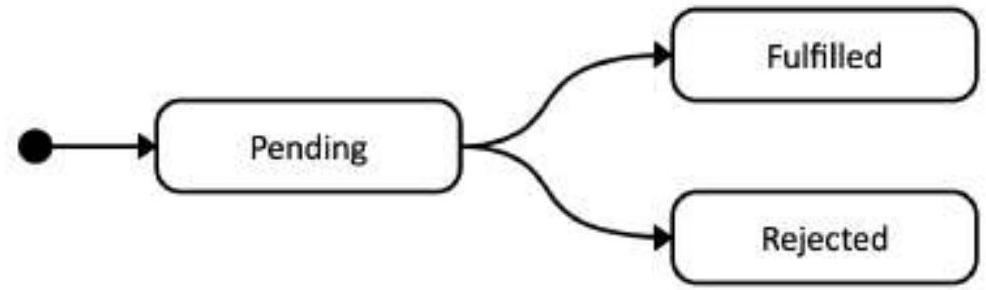
\includegraphics[width=0.8\linewidth]{images/2024_12_29_858f09cde51177c71657g-14}
\end{theorem}

\begin{corollary}{Promises Verknüpfen}
\begin{itemize}
  \item Then-Aufruf gibt selbst Promise zurück
  \item Catch-Aufruf ebenfalls, per Default erfüllt
  \item So können diese Aufrufe verkettet werden
  \item Promise, welche unmittelbar resolved wird: Promise.resolve (...)
  \item Promise, welche unmittelbar rejected wird: Promise.reject (...)
\end{itemize}
\end{corollary}

\begin{definition}{Promise.all()}
\begin{itemize}
  \item Erhält Array von Promises
  \item Erfüllt mit Array der Result, wenn alle erfüllt sind
  \item Zurückgewiesen sobald eine Promise zurückgewiesen wird
\end{itemize}
\end{definition}

\begin{definition}{Promise.race()}
\begin{itemize}
  \item Erhält Array von Promises
  \item Erfüllt sobald eine davon erfüllt ist
  \item Zurückgewiesen sobald eine davon zurückgewiesen wird
\end{itemize}
\end{definition}

\begin{KR}{Promise.all() und Promise.race()}
\begin{lstlisting}[language=JavaScript, style=basesmol]
// Promise.all
Promise.all([promise1, promise2])
    .then(results => {
        // Array mit allen Ergebnissen
    });

// Promise.race
Promise.race([promise1, promise2])
    .then(firstResult => {
        // Erstes erfuelltes Promise
    });
\end{lstlisting}
\end{KR}

\begin{definition}{Async/Await}
\begin{itemize}
  \item Syntaktischer Zucker für Promises
  \item Ersetzt Promise-Verkettung durch sequentielle Ausführung
  \item \texttt{async} markiert Funktion als asynchron
  \item \texttt{await} wartet auf Promise-Resolution
  \item \texttt{try/catch} für Fehlerbehandlung
  \item \texttt{Promise.all} kann durch parallele \texttt{await} ersetzt werden
  \item \texttt{await} gibt Wert von Promise zurück
  \item \texttt{await} kann nur in \texttt{async}-Funktionen verwendet werden
\end{itemize}
\end{definition}

\begin{KR}{Async/Await}
\begin{lstlisting}[language=JavaScript, style=basesmol]
// Async/Await Syntax
async function myAsync() {
    try {
        const result = await myPromise;
        // Erfolgsfall
    } catch (error) {
        // Fehlerfall
    }
}

// Async Funktion
async function getData() {
    try {
        const response = await fetch(url);
        const data = await response.json();
        return data;
    } catch (error) {
        console.error('Error:', error);
    }
}

// Parallele Ausfuehrung
async function getMultipleData() {
    const [data1, data2] = await Promise.all([
        getData(url1),
        getData(url2)
    ]);
    return { data1, data2 };
}
\end{lstlisting}
\end{KR}

\begin{code}{ASYNC/AWAIT}
\begin{lstlisting}[language=JavaScript, style=basesmol]
/* Bekanntes Beispiel */
const readHosts =() => {
    readFilePromise('/etc/hosts')
        .then(console.log)
        . catch(() => {
            console.log("Error reading file")
        })
}
/* Mit async/await */
const readHosts = async () => {
    try {
        console.log(await readFilePromise('/etc/hosts'))
    }
    catch (err) {
        console.log("Error reading file")
    }
}
\end{lstlisting}
Beispiel 2:
\begin{lstlisting}[language=JavaScript, style=basesmol]
function resolveAfter2Seconds (x) {
    return new Promise(resolve => {
        setTimeout(() => {
            resolve(x)
        }, 2000)
    })
}
async function add1(x) {
    var a = resolveAfter2Seconds(20)
    var b = resolveAfter2Seconds(30)
    return x + await a + await b
}
add1(10).then(console.log)
\end{lstlisting}
\end{code}

%TODO: add more examples for async/await and promises and event loop

\pagebreak

\subsection{Webserver}

\subsubsection{Server im Internet}
%TODO: add information about server in the internet

\subsubsection{File-Transfer (File Server)}


\begin{definition}{Web-Transfer-Protokolle}\\
    \textbf{File-Transfer:}
    \begin{itemize}
        \item FTP (File Transfer Protocol)
        \item SFTP (SSH File Transfer Protocol)
        \item Anwendungen mit GUI und Kommandozeile
    \end{itemize}

    \textbf{HTTP/HTTPS:}
    \begin{itemize}
        \item Standard-Ports: 80/443
        \item Request-Response Modell
        \item Stateless Protokoll
        \item HTTPS: Verschlüsselte Übertragung mittels SSL/TLS
    \end{itemize}
\end{definition}

\subsubsection{HTTP-Server}

\begin{corollary}{Ports}
    \begin{center}
    \begin{tabular}{|l|l|}
    \hline
    Port & Service \\
    \hline
    $\mathbf{20}$ & FTP - Data \\
    \hline
    $\mathbf{21}$ & FTP - Control \\
    \hline
    $\mathbf{22}$ & SSH Remote Login Protocol \\
    \hline
    $\mathbf{23}$ & Telnet \\
    \hline
    $\mathbf{25}$ & Simple Mail Transfer Protocol (SMTP) \\
    \hline
    $\mathbf{53}$ & Domain Name System (DNS) \\
    \hline
    $\mathbf{80}$ & HTTP \\
    \hline
    $\mathbf{443}$ & HTTPS \\
    \hline
    \end{tabular}
    \end{center}
\end{corollary}

\begin{theorem}{HTTP-Methoden}
    \begin{center}
    \begin{tabular}{|l|l|}
    \hline
    Methode & Verwendung \\
    \hline
    GET & Daten abrufen \\
    \hline
    POST & Neue Daten erstellen \\
    \hline
    PUT & Daten aktualisieren (komplett) \\
    \hline
    PATCH & Daten aktualisieren (teilweise) \\
    \hline
    DELETE & Daten löschen \\
    \hline
    \end{tabular}
    \end{center}
\end{theorem}

\begin{corollary}{HTTP Status Codes}
    \begin{center}
    \begin{tabular}{|l|l|}
    \hline
    Code & Bedeutung \\
    \hline
    200 & OK - Erfolgreich \\
    \hline
    201 & Created - Ressource erstellt \\
    \hline
    400 & Bad Request - Fehlerhafte Anfrage \\
    \hline
    401 & Unauthorized - Nicht authentifiziert \\
    \hline
    403 & Forbidden - Keine Berechtigung \\
    \hline
    404 & Not Found - Ressource nicht gefunden \\
    \hline
    500 & Internal Server Error - Serverfehler \\
    \hline
    \end{tabular}
    \end{center}
\end{corollary}
\columnbreak

\subsubsection{Node.js und Module}

\begin{concept}{Node.js}
    \begin{itemize}
        \item JavaScript Runtime basierend auf V8
        \item Event-driven und non-blocking I/O
        \item Großes Ökosystem (npm)
        \item Ideal für Netzwerk-Anwendungen
        \item REPL für interaktive Entwicklung
    \end{itemize}
\end{concept}

\begin{concept}{Module System}
    JavaScript verwendet verschiedene Modulsysteme:
    \begin{itemize}
        \item CommonJS (Node.js): \texttt{require}/\texttt{module.exports}
        \item ES Modules: \texttt{import}/\texttt{export}
    \end{itemize}
\end{concept}

\begin{KR}{Module Import/Export}
\begin{lstlisting}[language=JavaScript, style=basesmol]
// CommonJS (Node.js)
const fs = require('fs');
module.exports = { /* ... */ };

// ES Modules
import { function1, function2 } from './module.js';
export const variable = 42;
export default class MyClass { /* ... */ }
\end{lstlisting}
\end{KR}

% Error Handling
\begin{KR}{Error Handling}
\begin{lstlisting}[language=JavaScript, style=basesmol]
try {
    // Code der Fehler werfen konnte
    throw new Error('Something went wrong');
} catch (error) {
    // Fehlerbehandlung
    console.error(error.message);
} finally {
    // Wird immer ausgefuhrt
    cleanup();
}
\end{lstlisting}
\end{KR}

\begin{KR}{Module System}
\begin{lstlisting}[language=JavaScript, style=basesmol]
// CommonJS (Node.js)
const fs = require('fs');
module.exports = { /* ... */ };

// ES Modules
import { function1 } from './module.js';
export const variable = 42;
export default class MyClass { /* ... */ }

// package.json
{
    "type": "module",
    "dependencies": {
        "express": "^4.17.1"
    }
}
\end{lstlisting}
\end{KR}

\begin{formula}{NPM Commands}
    Wichtige npm Befehle:
    \begin{itemize}
        \item \texttt{npm init}: Projekt initialisieren
        \item \texttt{npm install}: Abhängigkeiten installieren
        \item \texttt{npm install --save package}: Produktiv-Dependency
        \item \texttt{npm install --save-dev package}: Entwicklungs-Dependency
        \item \texttt{npm run script}: Script ausführen
        \item \texttt{npm update}: Packages aktualisieren
    \end{itemize}
\end{formula}

\paragraph{Einfacher Webserver (Node.js)}

\begin{concept}{Node.js Webserver}
\begin{lstlisting}[language=JavaScript, style=basesmol]
const {createServer} = require("http")
Let server = createServer((request, response) => {
    response.writeHead(200, {"Content-Type": "text/html"})
    response.write(`
        <h1>Hello!</h1>
        <p>You asked for <code>${request.url}</code></p>`)
    response.end()
})
server.listen(8000)
console.log("Listening! (port 8000)")|
\end{lstlisting}
\end{concept}


\begin{code}{Einfacher Webclient}
\begin{lstlisting}[language=JavaScript, style=basesmol]
const {request} = require("http")
let requestStream = request({
    hostname: "eloquentjavascript.net",
        path: "/20_node.html",
        method: "GET"
        headers: {Accept: "text/html"}
}, response => {
        console.log("Server responded with status code", response.statusCode)
})
requestStream.end()
\end{lstlisting}
\end{code}

\begin{examplecode}{Server und Client mit Streams}
\begin{lstlisting}[language=JavaScript, style=basesmol]
const {createServer} = require("http")
createServer((request, response) => {
    response.writeHead(200, {"Content-Type": "text/plain"})
        request.on("data", chunk =>
            response.write(chunk.toString().toUpperCase()))
        request.on("end" , () => response.end())
    }).listen(8000)
\end{lstlisting}

\begin{lstlisting}[language=JavaScript, style=basesmol]
const {request} = require("http")
Let rq = request({
    hostname: "localhost",
    port: 8000,
    method: "POST"
}, response => {
    response.on("data", chunk =>
    process.stdout.write(chunk.toString()));
})
rq.write("Hello server\n")
rq.write("And good bye\n")
rq.end()
\end{lstlisting}
\end{examplecode}

\columnbreak

\subsubsection{REST API und Express.js}

\begin{definition}{REST API}
\begin{itemize}
  \item REST: Representational State Transfer
  \item Zugriff auf Ressourcen über ihre Adresse (URI)
  \item Kein Zustand: jede Anfrage komplett unabhängig
  \item Kein Bezug zu vorhergehenden Anfragen
  \item Alle nötigen Informationen in Anfrage enthalten
  \item Verwenden der HTTP-Methoden: GET , PUT , POST , ...
\end{itemize}
\end{definition}

\begin{concept}{Express.js}\\
    Express.js ist ein minimales, aber flexibles Framework für Web-apps. Es hat zahlreiche Utilities und Erweiterungen. 
    Express.js basiert auf Node.js.
    $\rightarrow$ http://expressjs.com
\end{concept}


\begin{KR}{Installation}
\begin{itemize}
  \item Der Schritt npm init fragt eine Reihe von Informationen (Projektname, Version, ...) zum Projekt ab
  \item Als Entry Point ist hier index.js voreingestellt
  \item Das kann zum Beispiel in app.js geändert werden.
\end{itemize}
\begin{lstlisting}[language=JavaScript, style=basesmol]
$ mkdir myapp
$ cd myapp
$ npm init
$ npm install express --save
\end{lstlisting}
\end{KR}

\begin{code}{Beispiel: Express Server}
\begin{lstlisting}[language=JavaScript, style=basesmol]
const express = require('express')
const app = express()
const port = 3000
app.get('/', (req, res) => {
        res.send('Hello World!')
})
app.listen(port, () => {
    console.log(`Example app listening at http://localhost:${port}`)
}})
\end{lstlisting}
\end{code}

\begin{KR}{Routing}
\begin{lstlisting}[language=JavaScript, style=basesmol]
app.get('/', function (req, res) {
    res.send('Hello World!')
})
app.post('/', function (req, res) {
    res.send('Got a POST request')
})
app.put('/user', function (req, res) {
    res.send('Got a PUT request at /user')
})
app.delete('/user', function (req, res) {
    res.send('Got a DELETE request at /user')
})
\end{lstlisting}
\end{KR}

\columnbreak

\subsection{Jasmine (Testing)}

\begin{concept}{Test-Driven Development}
    \begin{itemize}
        \item Tests vor Implementation schreiben
        \item Red-Green-Refactor Zyklus
        \item Tests als Spezifikation
        \item Bessere Code-Qualität
        \item Einfacheres Refactoring
    \end{itemize}
\end{concept}

\begin{KR}{Jasmine Tests}
\begin{lstlisting}[language=JavaScript, style=basesmol]
describe("Calculator", () => {
    let calc;
    
    beforeEach(() => {
        calc = new Calculator();
    });
    
    it("should add numbers", () => {
        expect(calc.add(1, 2)).toBe(3);
    });
    
    it("should throw on division by zero", () => {
        expect(() => {
            calc.divide(1, 0);
        }).toThrow();
    });
});
\end{lstlisting}
\end{KR}

\begin{formula}{Jasmine Matchers}
    \begin{itemize}
        \item \texttt{toBe()}: Strikte Gleichheit (===)
        \item \texttt{toEqual()}: Strukturelle Gleichheit
        \item \texttt{toContain()}: Array/String enthält Element
        \item \texttt{toBeDefined()}, \texttt{toBeUndefined()}
        \item \texttt{toBeTruthy()}, \texttt{toBeFalsy()}
        \item \texttt{toBeGreaterThan()}, \texttt{toBeLessThan()}
        \item \texttt{toMatch()}: RegExp Match
        \item \texttt{toThrow()}: Exception wird geworfen
    \end{itemize}
\end{formula}

\begin{KR}{Jasmine Setup}
\begin{lstlisting}[language=JavaScript, style=basesmol]
// Installation
npm install --save-dev jasmine

// jasmine.json
{
    "spec_dir": "spec",
    "spec_files": [
        "**/*[sS]pec.js"
    ],
    "helpers": [
        "helpers/**/*.js"
    ]
}

// Test ausfuehren
npx jasmine
\end{lstlisting}
\end{KR}

\begin{examplecode}{Beispiel (zugehörige Tests)}
\begin{lstlisting}[language=JavaScript, style=basesmol]
/* PlayerSpec.js - Auszug */
describe("when song has been paused", function() {
    beforeEach(function() {
        player.play(song)
        player.pause()
    })
    it("should indicate that the song is currently paused", function() {
        expect(player.isPlaying).toBeFalsy()
        /* demonstrates use of 'not' with a custom matcher */
        expect(player).not.toBePlaying(song)
    })
    it("should be possible to resume", function() {
        player.resume()
        expect(player.isPlaying).toBeTruthy()
        expect(player.currentlyPlayingSong) .toEqual(song)
    })
})
\end{lstlisting}
\end{examplecode}

\begin{code}{JASMINE: MATCHER}
\begin{lstlisting}[language=JavaScript, style=basesmol]
expect([1, 2, 3]).toEqual([1, 2, 3])
expect(12).toBeTruthy()
expect("").toBeFalsy()
expect("Hello planet").not.toContain("world")
expect(null).toBeNull()
expect(8).toBeGreaterThan(5)
expect(12.34).toBeCloseTo(12.3, 1)
expect("horse_ebooks.jpg") .toMatch(/\w+.(jpg|gif|png|svg)/i)
\end{lstlisting}
\end{code}

\begin{KR}{JASMINE: TESTS DURCHFÜHREN}
\begin{lstlisting}[language=bash, style=basesmol]
$ npx jasmine
Randomized with seed 03741
Started
......
5 specs, 0 failures
Finished in 0.014 seconds
Randomized with seed 03741 
    (jasmine --random=true --seed=03741)
\end{lstlisting}
\end{KR}

	\raggedcolumns
	\pagebreak
	\section{Browser Technologies}

\subsection{Document Object Model (DOM)}

\begin{concept}{DOM Structure}
    \begin{itemize}
        \item Tree representation of HTML document
        \item Each HTML element becomes a node
        \item Nodes can be elements, text, or attributes
        \item Provides API for dynamic manipulation
        \item Foundation for interactive web applications
    \end{itemize}
\end{concept}

\begin{KR}{DOM Manipulation}
\begin{lstlisting}[language=JavaScript, style=basesmol]
// Selecting elements
const element = document.getElementById('myId');
const elements = document.getElementsByClassName('myClass');
const element = document.querySelector('.myClass');
const elements = document.querySelectorAll('div.myClass');

// Creating elements
const div = document.createElement('div');
const text = document.createTextNode('Hello');
div.appendChild(text);

// Modifying elements
element.innerHTML = '<span>New content</span>';
element.textContent = 'New text';
element.setAttribute('class', 'newClass');
element.classList.add('newClass');
element.style.backgroundColor = 'red';

// Tree navigation
element.parentNode
element.childNodes
element.children
element.firstChild
element.nextSibling
\end{lstlisting}
\end{KR}

\subsection{Events}

\begin{definition}{Event Handling}
    Events represent interactions or state changes:
    \begin{itemize}
        \item User interactions (clicks, keyboard input)
        \item Document loading stages
        \item Network status changes
        \item Timer completions
    \end{itemize}
\end{definition}

\begin{KR}{Event Listeners}
\begin{lstlisting}[language=JavaScript, style=basesmol]
// Adding event listeners
element.addEventListener('click', (event) => {
    console.log('Clicked!', event);
    event.preventDefault();  // Prevent default behavior
    event.stopPropagation(); // Stop event bubbling
});

// Removing event listeners
const handler = (event) => {
    console.log('Handler');
};
element.addEventListener('click', handler);
element.removeEventListener('click', handler);

// Event delegation
document.addEventListener('click', (event) => {
    if (event.target.matches('.button')) {
        // Handle button clicks
    }
});
\end{lstlisting}
\end{KR}

\begin{formula}{Common Events}
    \begin{itemize}
        \item Mouse: \texttt{click}, \texttt{dblclick}, \texttt{mouseover}, \texttt{mouseout}
        \item Keyboard: \texttt{keydown}, \texttt{keyup}, \texttt{keypress}
        \item Form: \texttt{submit}, \texttt{change}, \texttt{input}, \texttt{focus}, \texttt{blur}
        \item Document: \texttt{DOMContentLoaded}, \texttt{load}
        \item Window: \texttt{resize}, \texttt{scroll}
    \end{itemize}
\end{formula}

\subsection{Browser APIs}

\begin{concept}{Web APIs}
    Modern browsers provide numerous APIs:
    \begin{itemize}
        \item Storage (localStorage, sessionStorage)
        \item Fetch (network requests)
        \item Canvas and WebGL (graphics)
        \item Web Workers (parallel processing)
        \item Geolocation
        \item WebSockets (real-time communication)
    \end{itemize}
\end{concept}

\begin{KR}{Web Storage}
\begin{lstlisting}[language=JavaScript, style=basesmol]
// localStorage (persists between sessions)
localStorage.setItem('key', 'value');
const value = localStorage.getItem('key');
localStorage.removeItem('key');
localStorage.clear();

// sessionStorage (cleared when session ends)
sessionStorage.setItem('key', 'value');
const value = sessionStorage.getItem('key');

// Storing objects
const user = { name: 'John', age: 30 };
localStorage.setItem('user', JSON.stringify(user));
const storedUser = JSON.parse(localStorage.getItem('user'));
\end{lstlisting}
\end{KR}

\begin{KR}{Fetch API}
\begin{lstlisting}[language=JavaScript, style=basesmol]
// GET request
fetch('https://api.example.com/data')
    .then(response => response.json())
    .then(data => console.log(data))
    .catch(error => console.error('Error:', error));

// POST request
fetch('https://api.example.com/data', {
    method: 'POST',
    headers: {
        'Content-Type': 'application/json',
    },
    body: JSON.stringify({
        name: 'John',
        age: 30
    })
})
.then(response => response.json())
.then(data => console.log(data));

// With async/await
async function fetchData() {
    try {
        const response = await fetch('https://api.example.com/data');
        const data = await response.json();
        console.log(data);
    } catch (error) {
        console.error('Error:', error);
    }
}
\end{lstlisting}
\end{KR}

\subsection{Forms and HTTP}

\begin{definition}{HTML Forms}
    Forms enable user input and data submission:
    \begin{itemize}
        \item \texttt{<form>} element with action and method
        \item Various input types (text, password, checkbox, etc.)
        \item Form validation (HTML5 and JavaScript)
        \item Data submission via GET or POST
    \end{itemize}
\end{definition}

\begin{KR}{Form Handling}
\begin{lstlisting}[language=JavaScript, style=basesmol]
// Form submission
const form = document.querySelector('form');
form.addEventListener('submit', async (event) => {
    event.preventDefault();
    
    const formData = new FormData(form);
    try {
        const response = await fetch('/submit', {
            method: 'POST',
            body: formData
        });
        const result = await response.json();
        console.log(result);
    } catch (error) {
        console.error('Error:', error);
    }
});

// Form validation
const input = document.querySelector('input');
input.addEventListener('input', (event) => {
    if (input.validity.typeMismatch) {
        input.setCustomValidity('Please enter a valid email');
    } else {
        input.setCustomValidity('');
    }
});
\end{lstlisting}
\end{KR}

\begin{formula}{HTTP Methods}
    \begin{center}
    \begin{tabular}{|l|l|}
    \hline
    \textbf{Method} & \textbf{Purpose} \\
    \hline
    GET & Retrieve data \\
    POST & Create new resource \\
    PUT & Update entire resource \\
    PATCH & Partial update \\
    DELETE & Remove resource \\
    \hline
    \end{tabular}
    \end{center}
\end{formula}

\subsection{Express.js}

\begin{concept}{Express Framework}
    Minimal web application framework for Node.js:
    \begin{itemize}
        \item Routing system
        \item Middleware support
        \item Static file serving
        \item Template engine integration
        \item Error handling
    \end{itemize}
\end{concept}

\begin{KR}{Express Basic Server}
\begin{lstlisting}[language=JavaScript, style=basesmol]
const express = require('express');
const app = express();

// Middleware
app.use(express.json());
app.use(express.urlencoded({ extended: true }));
app.use(express.static('public'));

// Routes
app.get('/', (req, res) => {
    res.send('Hello World');
});

app.post('/api/data', (req, res) => {
    const data = req.body;
    // Process data
    res.json({ success: true, data });
});

// Error handling
app.use((err, req, res, next) => {
    console.error(err.stack);
    res.status(500).send('Something broke!');
});

// Start server
app.listen(3000, () => {
    console.log('Server running on port 3000');
});
\end{lstlisting}
\end{KR}

\subsection{Security Considerations}

\begin{concept}{Web Security}
    Common security concerns:
    \begin{itemize}
        \item Cross-Site Scripting (XSS)
        \item Cross-Site Request Forgery (CSRF)
        \item SQL Injection
        \item Session Hijacking
        \item Man-in-the-Middle Attacks
    \end{itemize}
\end{concept}

\begin{KR}{Security Best Practices}
\begin{lstlisting}[language=JavaScript, style=basesmol]
// Input sanitization
const sanitizeHTML = require('sanitize-html');
const cleanHTML = sanitizeHTML(dirtyHTML);

// CSRF Protection
app.use(csrf());
<form>
    <input type="hidden" name="_csrf" value="<%= csrfToken %>">
</form>

// Secure cookies
app.use(session({
    secret: 'secret-key',
    cookie: {
        secure: true,
        httpOnly: true,
        sameSite: 'strict'
    }
}));

// CORS
app.use(cors({
    origin: 'https://trusted-domain.com',
    methods: ['GET', 'POST']
}));
\end{lstlisting}
\end{KR}
	\raggedcolumns
	\pagebreak
	\section{UI-Bibliotheken und Komponenten}

\begin{definition}{Overview}
\begin{itemize}
  \item Frameworks und Bibliotheken
  \item DOM-Scripting und Abstraktionen
  \item JSX und SJDON
  \item Eigene Bibliothek: SuiWeb
\end{itemize}
\end{definition}

\subsection{Frameworks und Bibliotheken}

\begin{definition}{Framework vs. Bibliothek}
    \begin{itemize}
        \item \textbf{Bibliothek}: 
            \begin{itemize}
                \item Kontrolle beim eigenen Programm
                \item Funktionen werden nach Bedarf verwendet
                \item Beispiel: jQuery
            \end{itemize}
            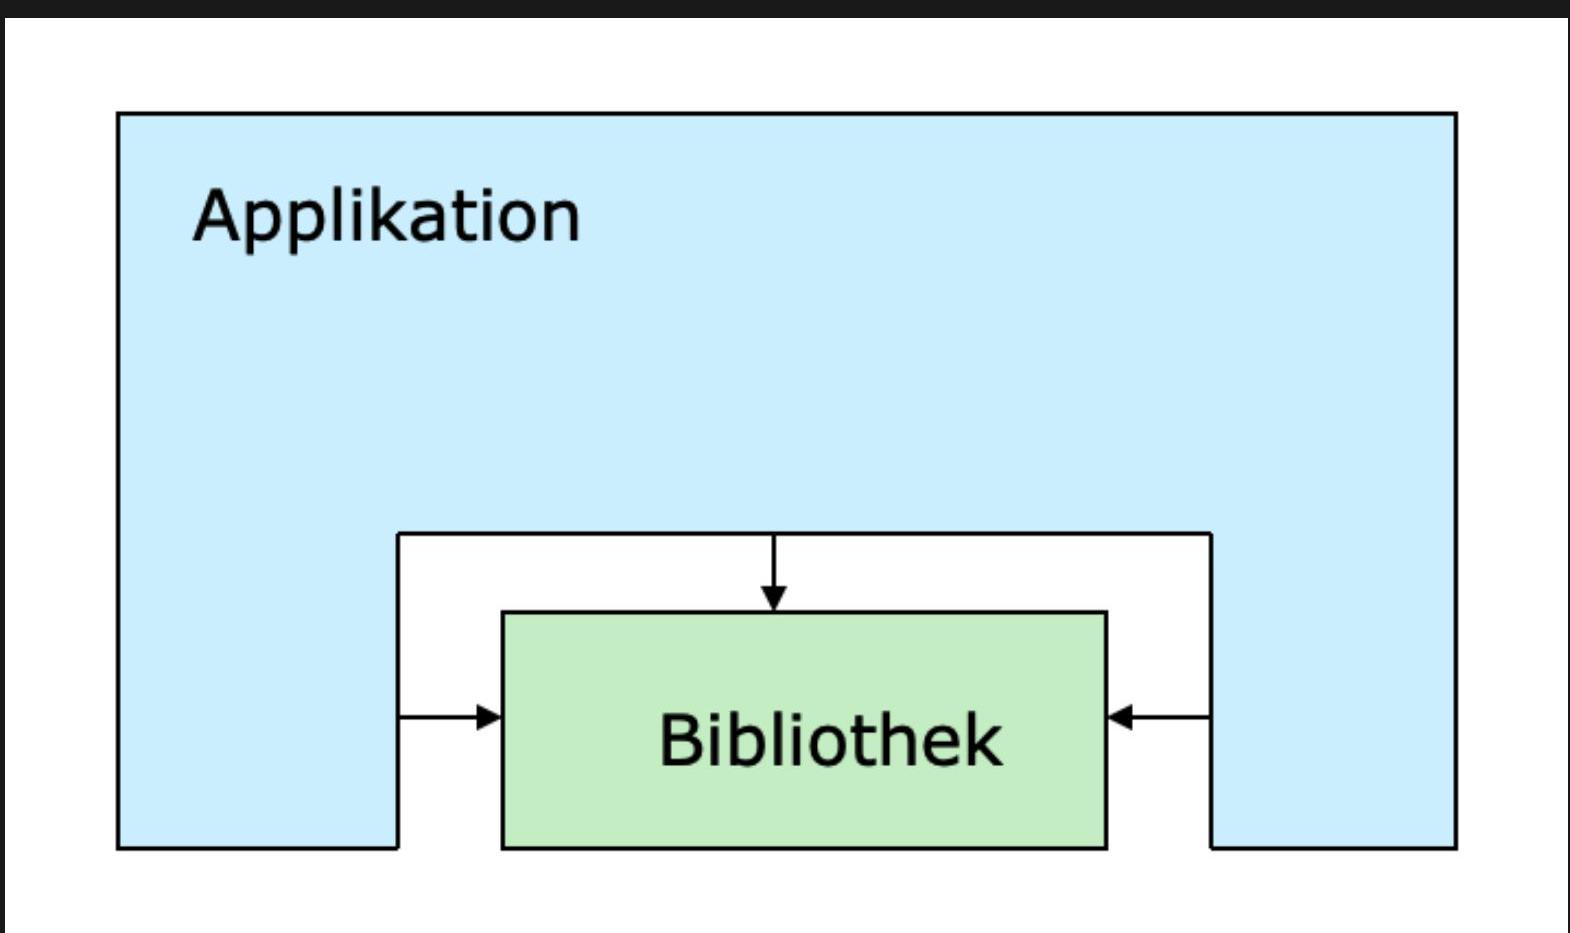
\includegraphics[width=0.5\linewidth]{images/2025_01_02_22162ee5453ad0230328g-04}
        \item \textbf{Framework}: 
            \begin{itemize}
                \item Rahmen für die Anwendung
                \item Kontrolle liegt beim Framework
                \item "Hollywood-Prinzip": don't call us, we'll call you
            \end{itemize}
            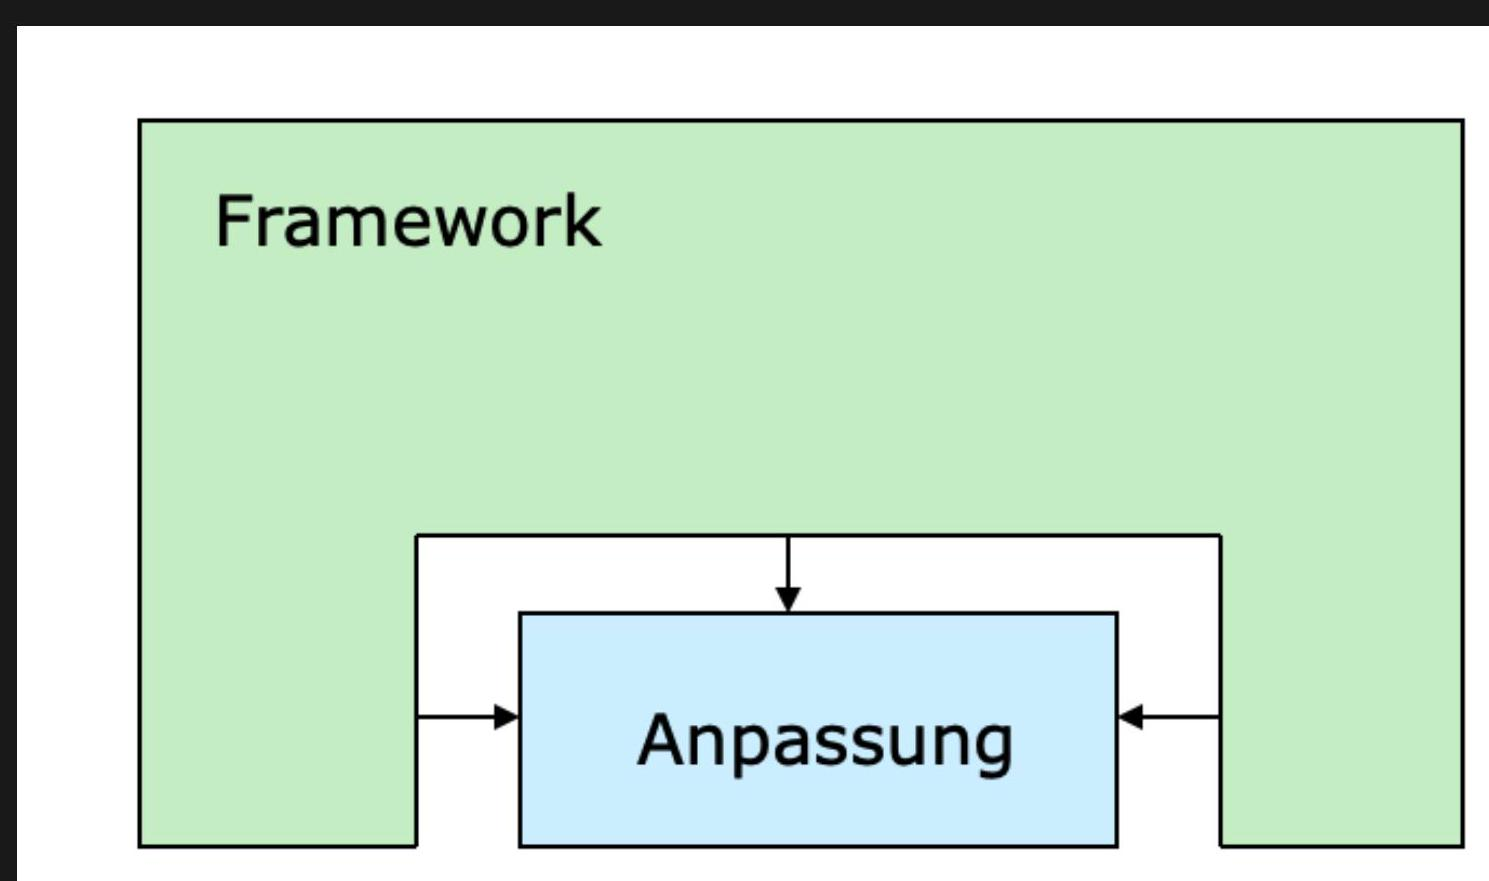
\includegraphics[width=0.5\linewidth]{images/2025_01_02_22162ee5453ad0230328g-05}
    \end{itemize}
\end{definition}

\begin{definition}{ANSÄTZE IM LAUF DER ZEIT}
\begin{itemize}
  \item Statische Webseiten
  \item Inhalte dynamisch generiert (CGI z.B. Shell Scripts, Perl)
  \item Serverseitig eingebettete Scriptsprachen (PHP)
  \item Client Scripting oder Applets (JavaScript, Java Applets, Flash)
  \item Enterprise Application Server (Java, Java EE)
  \item MVC Server-Applikationen (Rails, Django)
  \item JavaScript Server (Node.js)
  \item Single Page Applikationen (SPAs)
\end{itemize}
\end{definition}

\begin{definition}{SERVERSEITE}
\begin{itemize}
  \item Verschiedene Technologien möglich
  \item Zahlreiche Bibliotheken und Frameworks
  \item Verschiedene Architekturmuster
  \item Häufig: Model-View-Controller (MVC)
  \item Beispiel: Ruby on Rails
\end{itemize}
\end{definition}

\begin{concept}{Architektur}
\begin{itemize}
    \item \textbf{MVC (Model-View-Controller)}:
        \begin{itemize}
            \item Model: Repräsentiert Daten und Geschäftslogik, können Observer über Zustandsänderungen informieren
            \item View: Bildet UI (z.B. HTML/CSS), kommuniziert mit Controller
            \item Controller: Verarbeitet Eingaben (z.B. Clicks), aktualisiert Model
        \end{itemize}
    \item \textbf{Single Page Apps (SPAs)}:
        \begin{itemize}
            \item Vermeidet Neuladen von Seiten
            \item Inhalte dynamisch nachgeladen (Ajax, REST)
            \item Bessere Usability durch schnellere UI-Reaktion
        \end{itemize}
\end{itemize}
\end{concept}

\begin{concept}{Model-View-Controller (MVC)}
    \begin{itemize}
        \item \textbf{Models}
            \begin{itemize}
                \item Repräsentieren anwendungsspezifisches Wissen und Daten
                \item Ähnlich Klassen: User, Photo, Todo, Note
            \end{itemize}
        \item \textbf{Views}
            \begin{itemize}
                \item Bilden die Benutzerschnittstelle
                \item Meist HTML/CSS basiert
            \end{itemize}
        \item \textbf{Controllers}
            \begin{itemize}
                \item Verarbeiten Eingaben
                \item Aktualisieren Models
                \item Steuern View-Aktualisierung
            \end{itemize}
    \end{itemize}
\end{concept}

\begin{definition}{RUBY ON RAILS}
\begin{itemize}
  \item Serverseitiges Framework, basierend auf MVC
  \item Programmiersprache: Ruby\\
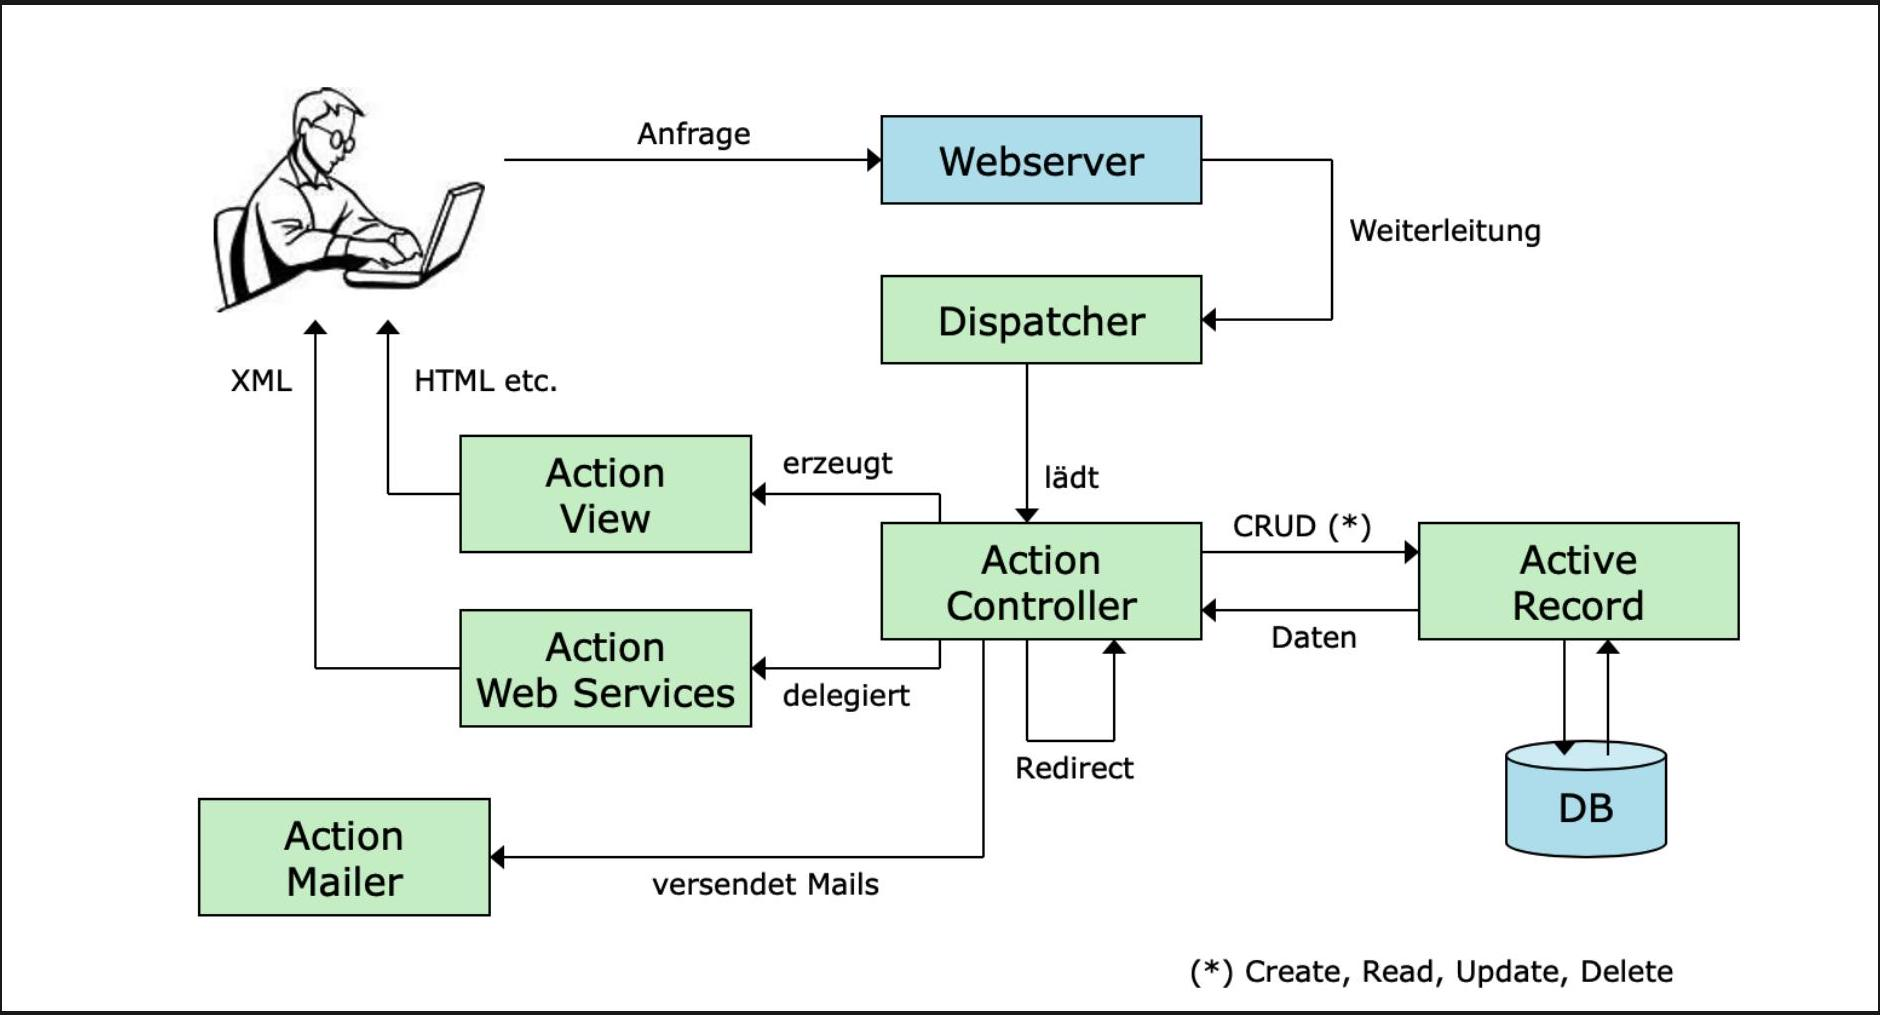
\includegraphics[width=\linewidth]{images/2025_01_02_22162ee5453ad0230328g-09}
\end{itemize}
\end{definition}

\begin{definition}{FOKUS AUF DIE CLIENT-SEITE}
\begin{itemize}
  \item Programmlogik Richtung Client verschoben
  \item Zunehmend komplexe User Interfaces
  \item Asynchrone Serveranfragen, z.B. mit Fetch
  \item Gute Architektur der Client-App wesentlich
  \item Diverse Frameworks und Bibliotheken zu diesem Zweck
\end{itemize}
\end{definition}

\begin{concept}{Komponentenbasierte Entwicklung}
    Grundprinzipien:
    \begin{itemize}
        \item UI in wiederverwendbare Komponenten aufteilen
        \item Klarer Datenfluss (Props down, Events up)
        \item Deklarativer Ansatz
        \item Komponenten können verschachtelt werden
        \item Zustandsverwaltung in Komponenten
        \item Container vs. Präsentations-Komponenten
    \end{itemize}
\end{concept}

\pagebreak


\subsection{DOM-Scripting und Abstraktionen}

\begin{definition}{DOM-SCRIPTING}
\begin{itemize}
  \item Zahlreiche Funktionen und Attribute verfügbar
  \item Programme werden schnell unübersichtlich
  \item Gesucht: geeignete Abstraktionen
\end{itemize}
\end{definition}

\begin{definition}{AUFGABE}
Liste aus einem Array erzeugen:
\begin{lstlisting}[language=JavaScript, style=basesmol]
/* gegeben: */
let data = ["Maria", "Hans", "Eva", "Peter"]
\end{lstlisting}

Entsprechendes Markup:
\begin{lstlisting}[language=HTML, style=basesmol]
<ul>
    <li>Maria</li>
    <li>Hans</li>
    <li>Eva</li>
    <li>Peter</li>
</ul>
\end{lstlisting}
\end{definition}

\begin{definition}{DOM-SCRIPTING}
\begin{lstlisting}[language=JavaScript, style=basesmol]
function List (data) {
    let node = document.createElement("ul")
    for (let item of data) {
        let elem = document.createElement("li")
        let elemText = document.createTextNode(item)
        elem.appendChild(elemText)
        node.appendChild(elem)
    }
    return node
}
\end{lstlisting}
\end{definition}

\begin{definition}{DOM-SCRIPTING VERBESSERT}
\begin{lstlisting}[language=JavaScript, style=basesmol]
function elt (type, attrs, ...children) {
    let node = document.createElement(type)
    Object.keys(attrs).forEach(key => {
        node.setAttribute(key, attrs[key])
    })
    for (let child of children) {
        if (typeof child != "string") node.appendChild(child)
        else node.appendChild(document.createTextNode(child))
    }
    return node
}
\end{lstlisting}

Damit vereinfachte List-Komponente möglich:
\begin{lstlisting}[language=JavaScript, style=basesmol]
function List (data) {
    return elt("ul", {}, ...data.map(item => elt("li", {}, item)))
}
\end{lstlisting}
\end{definition}

\subsubsection{JQUERY}

\begin{code}{jQuery List Implementation}
\begin{lstlisting}[language=JavaScript, style=basesmol]
function List (data) {
    return $("<ul>").append(...data.map(item => 
        $("<li>").text(item)))
}

function render (tree, elem) {
    while (elem.firstChild) { 
        elem.removeChild(elem.firstChild) 
    }
    $(elem).append(tree)
}
\end{lstlisting}
\end{code}

\begin{definition}{WEB COMPONENTS}
\begin{itemize}
  \item Möglichkeit, eigene Elemente zu definieren
  \item Implementiert mit HTML, CSS und JavaScript
  \item Implementierung im Shadow DOM verstecken
\end{itemize}

\begin{lstlisting}[language=HTML, style=basesmol]
<custom-progress-bar class="size">
<custom-progress-bar value="25">
<script>
    document.querySelector('.size').progress = 75;
</script>
\end{lstlisting}
\end{definition}

\subsection{JSX und SJDON}

\begin{definition}{JSX}
    \begin{itemize}
        \item XML-Syntax in JavaScript
        \item Muss zu JavaScript transpiliert werden
        \item HTML-Tags in Kleinbuchstaben
        \item Eigene Komponenten mit Großbuchstaben
        \item JavaScript-Ausdrücke in \{...\}
    \end{itemize}
\begin{lstlisting}[language=JavaScript, style=basesmol]
// JSX Komponente
const Welcome = ({name}) => (
    <div className="welcome">
        <h1>Hello, {name}</h1>
        <p>Welcome to our site!</p>
    </div>
);

// Verwendung
const element = <Welcome name="Alice" />;
\end{lstlisting}
\end{definition}

\begin{definition}{SJDON}
    Simple JavaScript DOM Notation:
    \begin{itemize}
        \item Alternative zu JSX
        \item Verwendet pure JavaScript Arrays und Objekte
        \item Kein Kompilierungsschritt nötig
        \item Array-basierte Notation
    \end{itemize}
\begin{lstlisting}[language=JavaScript, style=basesmol]
// SJDON Komponente
const Welcome = ({name}) => [
    "div", {className: "welcome"},
    ["h1", `Hello, ${name}`],
    ["p", "Welcome to our site!"]
];

// Verwendung
const element = [Welcome, {name: "Alice"}];
\end{lstlisting}
\end{definition}

\begin{KR}{Vergleich JSX und SJDON}
\begin{lstlisting}[language=JavaScript, style=basesmol]
// JSX
const element = (
    <div style={{background: 'salmon'}}>
        <h1>Hello World</h1>
        <h2 style={{textAlign: 'right'}}>
            from Web Framework
        </h2>
    </div>
);

// SJDON
const element = [
    "div", {style: "background:salmon"},
    ["h1", "Hello World"],
    ["h2", {style: "text-align:right"}, 
        "from Web Framework"]
];
\end{lstlisting}
\end{KR}

\pagebreak

\subsection{SuiWeb Framework}

\begin{concept}{SuiWeb Grundkonzepte}
    Simple User Interface Toolkit for Web Exercises:
    \begin{itemize}
        \item Komponentenbasiert wie React
        \item Unterstützt JSX und SJDON
        \item Datengesteuert mit Props und State
        \item Vereinfachte Implementation für Lernzwecke
        \item Props sind read-only
        \item State für veränderliche Daten
    \end{itemize}
\end{concept}

\subsubsection{State Management}

\begin{formula}{State Management}
    Zustandsverwaltung in SuiWeb:
    \begin{itemize}
        \item \texttt{useState} Hook für lokalen Zustand
        \item State Updates lösen Re-Rendering aus
        \item Asynchrone Updates werden gequeued
        \item Props sind read-only
    \end{itemize}
\end{formula}

\begin{concept}{State Hook}
    \begin{itemize}
        \item Zustandsverwaltung in Funktionskomponenten
        \item Initialisierung mit useState Hook
        \item State Updates lösen Re-Rendering aus
        \item Asynchrone Updates werden gequeued
    \end{itemize}
\end{concept}

\begin{KR}{State Verwaltung}
\begin{lstlisting}[language=JavaScript, style=basesmol]
const Counter = () => {
    // State initialisieren
    const [count, setCount] = useState(0);
    
    // Event Handler
    const increment = () => setCount(count + 1);
    const decrement = () => setCount(count - 1);
    
    return [
        "div",
        ["button", {onclick: decrement}, "-"],
        ["span", count],
        ["button", {onclick: increment}, "+"]
    ];
};

// Komplexere State Objekte
const Form = () => {
    const [state, setState] = useState({
        username: '',
        email: '',
        isValid: false
    });
    
    const updateField = (field, value) => {
        setState({
            ...state,
            [field]: value
        });
    };
};
\end{lstlisting}
\end{KR}

\begin{KR}{Kontrollierte Eingabefelder}
\begin{lstlisting}[language=JavaScript, style=basesmol]
const InputForm = () => {
    const [text, setText] = useState("");
    
    return [
        "form",
        ["input", {
            type: "text",
            value: text,
            oninput: e => setText(e.target.value)
        }],
        ["p", "Eingabe: ", text]
    ];
};
\end{lstlisting}
\end{KR}

\subsubsection{Komponenten-Design}

\begin{concept}{Container Components}
    \begin{itemize}
        \item Trennung von Daten und Darstellung
        \item Container kümmern sich um:
            \begin{itemize}
                \item Datenbeschaffung
                \item Zustandsverwaltung
                \item Event Handling
            \end{itemize}
        \item Präsentationskomponenten sind zustandslos
    \end{itemize}
\end{concept}

\begin{formula}{Component Design Principles}
    \begin{itemize}
        \item Single Responsibility Principle
        \item DRY (Don't Repeat Yourself)
        \item KISS (Keep It Simple, Stupid)
        \item Lifting State Up
        \item Props down, Events up
        \item Komposition über Vererbung
    \end{itemize}
\end{formula}

\begin{theorem}{Best Practices}
    Grundprinzipien für gutes Komponenten-Design:
    \begin{itemize}
        \item Single Responsibility Principle
        \item Trennung von Container und Präsentation
        \item Vermeidung von tiefer Verschachtelung
        \item Wiederverwendbarkeit fördern
        \item Klare Props-Schnittstelle
    \end{itemize}
\end{theorem}

\begin{KR}{Komponenten-Struktur}
\begin{lstlisting}[language=JavaScript, style=basesmol]
// Container Komponente
const UserContainer = () => {
    const [user, setUser] = useState(null);
    useEffect(() => {
        fetchUser().then(setUser);
    }, []);
    
    return [UserProfile, {user}];
};
// Praesentations-Komponente
const UserProfile = ({user}) => {
    if (!user) return ["div", "Loading..."];
    return [
        "div",
        ["h2", user.name],
        ["p", user.email],
        [UserDetails, {details: user.details}]
    ];
};
\end{lstlisting}
\end{KR}

\begin{KR}{Komponenten in SuiWeb}
\begin{lstlisting}[language=JavaScript, style=basesmol]
// Einfache Komponente
const MyButton = ({onClick, children}) => [
    "button",
    {
        onclick: onClick,
        style: "background: khaki"
    },
    ...children
];
// Komponente mit State
const Counter = () => {
    const [count, setCount] = useState(0);
    return [
        "div",
        ["button", 
            {onclick: () => setCount(count + 1)},
            `Count: ${count}`
        ]
    ];
};
\end{lstlisting}
\end{KR}

\begin{KR}{Container Komponente}
\begin{lstlisting}[language=JavaScript, style=basesmol]
const TodoContainer = () => {
    const [todos, setTodos] = useState([]);
    // Daten laden
    if (todos.length === 0) {
        fetchTodos().then(data => setTodos(data));
    }
    // Event Handler
    const addTodo = (text) => {
        setTodos([...todos, {
            id: Date.now(),
            text,
            completed: false
        }]);
    };
    const toggleTodo = (id) => {
        setTodos(todos.map(todo =>
            todo.id === id
                ? {...todo, completed: !todo.completed}
                : todo
        ));
    };
    // Render Praesentationskomponente
    return [TodoList, {
        todos,
        onToggle: toggleTodo,
        onAdd: addTodo
    }];
};
// Praesentationskomponente
const TodoList = ({todos, onToggle, onAdd}) => [
    "div",
    [TodoForm, {onAdd}],
    ["ul",
        ...todos.map(todo => [
            TodoItem, {
                key: todo.id,
                todo,
                onToggle
            }
        ])
    ]
];
\end{lstlisting}
\end{KR}

\begin{KR}{Container Komponenten}
\begin{lstlisting}[language=JavaScript, style=basesmol]
const MyContainer = () => {
    let initialState = { items: ["Loading..."] };
    let [state, setState] = useState(initialState);
    if (state === initialState) {
        fetchData()
            .then(items => setState({items}));
    }
    return [
        MyList, 
        {items: state.items}
    ];
};
\end{lstlisting}
\end{KR}

\begin{concept}{Event Handling}
    Behandlung von Benutzerinteraktionen:
    \begin{itemize}
        \item Events als Props übergeben
        \item Callback-Funktionen für Events
        \item State Updates in Event Handlern
        \item Vermeidung von direkter DOM-Manipulation
    \end{itemize}
\end{concept}

\begin{KR}{Event Handling Beispiel}
\begin{lstlisting}[language=JavaScript, style=basesmol]
const TodoList = () => {
    const [todos, setTodos] = useState([]);
    const addTodo = (text) => {
        setTodos([...todos, {
            id: Date.now(),
            text,
            completed: false
        }]);
    };
    const toggleTodo = (id) => {
        setTodos(todos.map(todo =>
            todo.id === id
                ? {...todo, completed: !todo.completed}
                : todo
        ));
    };
    return [
        "div",
        [TodoForm, {onSubmit: addTodo}],
        [TodoItems, {
            items: todos,
            onToggle: toggleTodo
        }]
    ];
};
\end{lstlisting}
\end{KR}

\begin{corollary}{Optimierungen}
    Möglichkeiten zur Performanzverbesserung:
    \begin{itemize}
        \item Virtuelles DOM für effizientes Re-Rendering
        \item Batching von State Updates
        \item Memoization von Komponenten
        \item Lazy Loading von Komponenten
    \end{itemize}
\end{corollary}

\subsubsection{Styling in SuiWeb}

\begin{concept}{Styling in SuiWeb}
    Verschiedene Möglichkeiten für Styles:
    \begin{itemize}
        \item Inline Styles als Strings
        \item Style-Objekte
        \item Arrays von Style-Objekten
        \item Externe CSS-Klassen
    \end{itemize}
\end{concept}

\begin{formula}{Styling Best Practices}
    \begin{itemize}
        \item Konsistente Styling-Methode verwenden
        \item Styles in separaten Objekten/Modulen
        \item Wiederverwendbare Style-Definitionen
        \item Responsive Design beachten
        \item CSS-Klassen für komplexe Styles
    \end{itemize}
\end{formula}

\begin{KR}{Style Optionen}
\begin{lstlisting}[language=JavaScript, style=basesmol]
// String Style
["div", {style: "color: blue; font-size: 16px"}]
// Style Objekt
const styles = {
    container: {
        backgroundColor: "lightgray",
        padding: "10px"
    },
    text: {
        color: "darkblue",
        fontSize: "14px"
    }
};
// Kombinierte Styles
["div", {
    style: [
        styles.container,
        {borderRadius: "5px"}
    ]
}]
\end{lstlisting}
\end{KR}

\subsection{Von SuiWeb zu React}

\begin{concept}{React.js Kernkonzepte}
    \begin{itemize}
        \item JavaScript-Bibliothek für User Interfaces
        \item Entwickelt von Facebook (2013)
        \item Hauptprinzipien:
            \begin{itemize}
                \item Deklarativ
                \item Komponentenbasiert
                \item Learn Once, Write Anywhere
                \item Virtual DOM für effizientes Rendering
                \item Unidirektionaler Datenfluss
            \end{itemize}
    \end{itemize}
\end{concept}

\begin{KR}{React Components}
\begin{lstlisting}[language=JavaScript, style=basesmol]
// Function Component
const Welcome = ({name}) => {
    return <h1>Hello, {name}</h1>;
};
// State Hook
const Counter = () => {
    const [count, setCount] = useState(0);
    
    return (
        <div>
            <p>Count: {count}</p>
            <button onClick={() => setCount(count + 1)}>
                Increment
            </button>
        </div>
    );
};
// Effect Hook
const DataFetcher = () => {
    const [data, setData] = useState(null);
    
    useEffect(() => {
        fetchData().then(setData);
    }, []);
    
    return data ? <DisplayData data={data} /> : <Loading />;
};
\end{lstlisting}
\end{KR}

\subsection{Performance Optimierung}

\begin{concept}{Rendering Optimierung}
    \begin{itemize}
        \item Virtuelles DOM für effizientes Re-Rendering
        \item Batching von State Updates
        \item Memoization von Komponenten
        \item Lazy Loading
        \item Key Prop für Listen-Elemente
    \end{itemize}
\end{concept}

\begin{KR}{Performance Best Practices}
\begin{lstlisting}[language=JavaScript, style=basesmol]
// Effiziente Listen-Rendering
const List = ({items}) => [
    "ul",
    ...items.map(item => [
        "li",
        {key: item.id},  // Wichtig fuer Performance
        item.text
    ])
];
// Lazy Loading
const LazyComponent = async () => {
    const module = await import('./Component.js');
    return module.default;
};
\end{lstlisting}
\end{KR}
	\pagebreak
    \section{Wrap-up}

\subsection{Überblick des Kurses}

\begin{formula}{Hauptthemen}
    \begin{enumerate}
        \item JavaScript Grundlagen
            \begin{itemize}
                \item Sprache und Syntax
                \item Objekte und Arrays
                \item Funktionen und Prototypen 
                \item Asynchrone Programmierung
                \item Node.js und Module
            \end{itemize}
        \item Browser-Technologien
            \begin{itemize}
                \item DOM Manipulation
                \item Events und Event Handling
                \item Web Storage
                \item Canvas und SVG
                \item Client-Server Kommunikation
            \end{itemize}
        \item UI-Bibliotheken
            \begin{itemize}
                \item Komponentenbasierte Entwicklung
                \item JSX und SJDON
                \item State Management
                \item SuiWeb Framework
            \end{itemize}
    \end{enumerate}
\end{formula}



\subsection{Weiterführende Themen}

\begin{concept}{Modern Web Development}
    \begin{itemize}
        \item Mobile Development
            \begin{itemize}
                \item Responsive Design
                \item Progressive Web Apps
                \item React Native
            \end{itemize}
        \item Performance
            \begin{itemize}
                \item WebAssembly (WASM)
                \item Code Splitting
                \item Service Workers
            \end{itemize}
        \item Alternative Technologien
            \begin{itemize}
                \item TypeScript
                \item Svelte
                \item Vue.js
            \end{itemize}
    \end{itemize}
\end{concept}

\begin{formula}{JavaScript Ecosystem}
    Wichtige Tools und Frameworks:
    \begin{itemize}
        \item \textbf{Build Tools:}
            \begin{itemize}
                \item Webpack
                \item Vite
                \item Babel
            \end{itemize}
        \item \textbf{Testing:}
            \begin{itemize}
                \item Jest
                \item Testing Library
                \item Cypress
            \end{itemize}
        \item \textbf{State Management:}
            \begin{itemize}
                \item Redux
                \item MobX
                \item Zustand
            \end{itemize}
    \end{itemize}
\end{formula}

\begin{KR}{Best Practices}
    Wichtige Prinzipien für die Web-Entwicklung:
    \begin{itemize}
        \item Clean Code
            \begin{itemize}
                \item DRY (Don't Repeat Yourself)
                \item KISS (Keep It Simple, Stupid)
                \item Single Responsibility Principle
            \end{itemize}
        \item Performance
            \begin{itemize}
                \item Lazy Loading
                \item Code Splitting
                \item Caching Strategien
            \end{itemize}
        \item Security
            \begin{itemize}
                \item HTTPS
                \item CORS
                \item Content Security Policy
            \end{itemize}
    \end{itemize}
\end{KR}

\subsection{Ressourcen}

\begin{concept}{Weiterführende Materialien}
    \begin{itemize}
        \item \textbf{Dokumentation:}
            \begin{itemize}
                \item MDN Web Docs: \url{https://developer.mozilla.org}
                \item React Docs: \url{https://react.dev}
                \item Node.js Docs: \url{https://nodejs.org/docs}
            \end{itemize}
        \item \textbf{Bücher:}
            \begin{itemize}
                \item "Eloquent JavaScript" von Marijn Haverbeke
                \item "You Don't Know JS" von Kyle Simpson
                \item "JavaScript: The Good Parts" von Douglas Crockford
            \end{itemize}
        \item \textbf{Online Kurse:}
            \begin{itemize}
                \item freeCodeCamp
                \item Frontend Masters
                \item Egghead.io
            \end{itemize}
    \end{itemize}
\end{concept}

\begin{theorem}{Kursabschluss}
    Wichtige Lernergebnisse:
    \begin{itemize}
        \item Solides Verständnis von JavaScript
        \item Beherrschung der Browser-APIs
        \item Komponentenbasierte Entwicklung
        \item Moderne Web-Entwicklungspraktiken
        \item Basis für fortgeschrittene Themen
    \end{itemize}
\end{theorem}
	\raggedcolumns
	%\pagebreak
    %\section{Übungsaufgaben}

\subsection{JavaScript Grundlagen}

\begin{example2}{Datentypen und Operatoren}
    \textbf{Aufgabe 1:} Was ist die Ausgabe folgender Ausdrücke?
    \begin{lstlisting}[language=JavaScript, style=basesmol]
typeof NaN
typeof []
typeof null
typeof undefined
[] == false
null === undefined
"5" + 3
"5" - 3
    \end{lstlisting}
    
    \textbf{Lösung:}
    \begin{lstlisting}[language=JavaScript, style=basesmol]
"number"     // NaN ist vom Typ number
"object"     // Arrays sind Objekte
"object"     // null ist historisch ein Objekt
"undefined"  // undefined ist ein eigener Typ
true         // [] wird zu 0 konvertiert
false        // === vergleicht auch Typen
"53"         // String-Konkatenation
2            // Numerische Subtraktion
    \end{lstlisting}
\end{example2}

\begin{example2}{Funktionen und Scoping}
    \textbf{Aufgabe 2:} Was ist die Ausgabe dieses Codes?
    \begin{lstlisting}[language=JavaScript, style=basesmol]
let x = 1;
const f = () => {
    let x = 2;
    return {
        getX: () => x,
        setX: (val) => { x = val; }
    };
};
const obj = f();
console.log(x);        // ?
console.log(obj.getX()); // ?
obj.setX(3);
console.log(obj.getX()); // ?
console.log(x);        // ?
    \end{lstlisting}
    
    \textbf{Lösung:}
    \begin{lstlisting}[language=JavaScript, style=basesmol]
1    // Globales x bleibt 1
2    // Closure hat Zugriff auf lokales x
3    // Lokales x wird auf 3 gesetzt
1    // Globales x bleibt unveraendert
    \end{lstlisting}
\end{example2}

\subsection{DOM und Events}

\begin{example2}{DOM Manipulation}
    \textbf{Aufgabe 3:} Erstellen Sie eine Funktion, die eine ToDo-Liste verwaltet.
    \begin{lstlisting}[language=JavaScript, style=basesmol]
function createTodoList(containerId) {
    // Container finden
    const container = document.getElementById(containerId);
    
    // Input und Liste erstellen
    const input = document.createElement('input');
    const button = document.createElement('button');
    const list = document.createElement('ul');
    
    // Button konfigurieren
    button.textContent = 'Add';
    button.onclick = () => {
        if (input.value.trim()) {
            const li = document.createElement('li');
            li.textContent = input.value;
            list.appendChild(li);
            input.value = '';
        }
    };
    
    // Elemente zusammenfuegen
    container.appendChild(input);
    container.appendChild(button);
    container.appendChild(list);
}
    \end{lstlisting}
\end{example2}

\begin{example2}{Event Handling}
    \textbf{Aufgabe 4:} Implementieren Sie einen Klick-Zähler mit Event Delegation.
    \begin{lstlisting}[language=JavaScript, style=basesmol]
document.getElementById('container').addEventListener('click', 
    (e) => {
        if (e.target.matches('button')) {
            const count = (
                parseInt(e.target.dataset.count) || 0
            ) + 1;
            e.target.dataset.count = count;
            e.target.textContent = `Clicked ${count} times`;
        }
    }
);
    \end{lstlisting}
\end{example2}

\subsection{Client-Server Kommunikation}

\begin{example2}{Fetch API}
    \textbf{Aufgabe 5:} Implementieren Sie eine Funktion für API-Requests.
    \begin{lstlisting}[language=JavaScript, style=basesmol]
async function apiRequest(url, method = 'GET', data = null) {
    const options = {
        method,
        headers: {
            'Content-Type': 'application/json'
        }
    };
    
    if (data) {
        options.body = JSON.stringify(data);
    }
    
    try {
        const response = await fetch(url, options);
        if (!response.ok) {
            throw new Error(`HTTP error: ${response.status}`);
        }
        return await response.json();
    } catch (error) {
        console.error('API request failed:', error);
        throw error;
    }
}
    \end{lstlisting}
\end{example2}

\begin{example2}{Formular-Validierung}
    \textbf{Aufgabe 6:} Erstellen Sie eine Formular-Validierung.
    \begin{lstlisting}[language=JavaScript, style=basesmol]
function validateForm(formId) {
    const form = document.getElementById(formId);
    
    form.addEventListener('submit', (e) => {
        e.preventDefault();
        
        const formData = new FormData(form);
        const errors = [];
        
        // Email validieren
        const email = formData.get('email');
        if (!email.includes('@')) {
            errors.push('Invalid email');
        }
        
        // Passwort validieren
        const password = formData.get('password');
        if (password.length < 8) {
            errors.push('Password too short');
        }
        
        if (errors.length === 0) {
            // Form submission logic
            console.log('Form valid, submitting...');
            form.submit();
        } else {
            alert(errors.join('\n'));
        }
    });
}
    \end{lstlisting}
\end{example2}

\subsection{UI-Komponenten}

\begin{example2}{SuiWeb Komponente}
    \textbf{Aufgabe 7:} Erstellen Sie eine Counter-Komponente mit SuiWeb.
    \begin{lstlisting}[language=JavaScript, style=basesmol]
const Counter = () => {
    const [count, setCount] = useState(0);
    
    return [
        "div",
        ["h2", `Count: ${count}`],
        ["button", 
            {onclick: () => setCount(count + 1)},
            "Increment"
        ],
        ["button", 
            {onclick: () => setCount(count - 1)},
            "Decrement"
        ]
    ];
};
    \end{lstlisting}
\end{example2}

\begin{example2}{Container Component}
    \textbf{Aufgabe 8:} Implementieren Sie eine UserList-Komponente.
    \begin{lstlisting}[language=JavaScript, style=basesmol]
const UserList = () => {
    const [users, setUsers] = useState([]);
    const [loading, setLoading] = useState(true);
    
    if (loading) {
        fetchUsers()
            .then(data => {
                setUsers(data);
                setLoading(false);
            })
            .catch(error => {
                console.error(error);
                setLoading(false);
            });
    }
    
    if (loading) {
        return ["div", "Loading..."];
    }
    
    return [
        "div",
        ["h2", "Users"],
        ["ul", 
            ...users.map(user => 
                ["li", `${user.name} (${user.email})`)
            ]
        ]
    ];
};
    \end{lstlisting}
\end{example2}

\subsection{Theoriefragen}

\begin{example2}{Konzeptfragen}
    \textbf{1. Erklären Sie den Unterschied zwischen == und === in JavaScript.}
    
    Antwort: == vergleicht Werte mit Typumwandlung, === vergleicht Werte und Typen ohne Umwandlung.
    
    \textbf{2. Was ist Event Bubbling?}
    
    Antwort: Events werden von dem auslösenden Element durch den DOM-Baum nach oben weitergeleitet.
    
    \textbf{3. Was ist der Unterschied zwischen localStorage und sessionStorage?}
    
    Antwort: localStorage persistiert Daten auch nach Schließen des Browsers, sessionStorage nur während der Session.
    
    \textbf{4. Erklären Sie den Unterschied zwischen synchronem und asynchronem Code.}
    
    Antwort: Synchroner Code wird sequentiell ausgeführt, asynchroner Code ermöglicht parallele Ausführung ohne Blockierung.
\end{example2}

\subsection{Praktische Aufgaben}

\begin{example2}{Implementierungsaufgaben}
    \textbf{1. Implementieren Sie eine Funktion zur Deep Copy von Objekten.}
    
    \textbf{2. Erstellen Sie eine Funktion, die prüft ob ein String ein Palindrom ist.}
    
    \textbf{3. Implementieren Sie eine debounce-Funktion.}
    
    \textbf{4. Erstellen Sie eine Komponente für einen Image Slider.}
\end{example2}

\begin{example2}{Debugging-Aufgaben}
    \textbf{1. Finden Sie den Fehler im folgenden Code:}
    \begin{lstlisting}[language=JavaScript, style=basesmol]
const getData = () => {
    fetch('api/data')
        .then(response => response.json())
        .then(data => {
            return data;
        });
}
// Warum kommt undefined zurueck?
    \end{lstlisting}
    
    Antwort: Die Funktion hat kein explizites return Statement. Sie sollte entweder async/await verwenden oder die Promise zurückgeben.
\end{example2}

	%\raggedcolumns
	%\pagebreak
	%\section{Example Exercises}

\subsection{JavaScript Fundamentals}

\begin{example2}{Basic Array Manipulation}
Write a function that takes an array of numbers and returns a new array containing only the even numbers, doubled.

\begin{lstlisting}[language=JavaScript, style=basesmol]
// Example solution
function processArray(numbers) {
    return numbers
        .filter(num => num % 2 === 0)
        .map(num => num * 2);
}

// Test
console.log(processArray([1, 2, 3, 4, 5, 6])); // [4, 8, 12]
\end{lstlisting}
\end{example2}

\begin{example2}{Closure Implementation}
Create a function that generates unique IDs with a given prefix. Each call should return a new ID with an incrementing number.

\begin{lstlisting}[language=JavaScript, style=basesmol]
// Example solution
function createIdGenerator(prefix) {
    let counter = 0;
    return function() {
        counter++;
        return `${prefix}${counter}`;
    };
}

// Test
const generateUserId = createIdGenerator('user_');
console.log(generateUserId()); // "user_1"
console.log(generateUserId()); // "user_2"
\end{lstlisting}
\end{example2}

\begin{example2}{Async Programming}
Write an async function that fetches user data from two different endpoints and combines them. Handle potential errors appropriately.

\begin{lstlisting}[language=JavaScript, style=basesmol]
async function getUserData(userId) {
    try {
        const [profile, posts] = await Promise.all([
            fetch(`/api/profile/${userId}`).then(r => r.json()),
            fetch(`/api/posts/${userId}`).then(r => r.json())
        ]);
        
        return {
            ...profile,
            posts: posts
        };
    } catch (error) {
        console.error('Failed to fetch user data:', error);
        throw new Error('Failed to load user data');
    }
}
\end{lstlisting}
\end{example2}

\subsection{DOM Manipulation}

\begin{example2}{Dynamic List Creation}
Write a function that takes an array of items and creates a numbered list in the DOM. Add a button to each item that removes it from the list.

\begin{lstlisting}[language=JavaScript, style=basesmol]
function createList(items, containerId) {
    const container = document.getElementById(containerId);
    const ul = document.createElement('ul');
    
    items.forEach((item, index) => {
        const li = document.createElement('li');
        li.textContent = `${index + 1}. ${item} `;
        
        const button = document.createElement('button');
        button.textContent = 'Remove';
        button.onclick = () => li.remove();
        
        li.appendChild(button);
        ul.appendChild(li);
    });
    
    container.appendChild(ul);
}
\end{lstlisting}
\end{example2}

\subsection{Component Implementation}

\begin{example2}{Form Component}
Create a form component in SuiWeb that handles user input with validation and submits data to a server.

\begin{lstlisting}[language=JavaScript, style=basesmol]
const UserForm = () => {
    const [formData, setFormData] = useState({
        username: '',
        email: ''
    });
    const [errors, setErrors] = useState({});
    
    const validate = () => {
        const newErrors = {};
        if (!formData.username) {
            newErrors.username = 'Username is required';
        }
        if (!formData.email.includes('@')) {
            newErrors.email = 'Valid email is required';
        }
        setErrors(newErrors);
        return Object.keys(newErrors).length === 0;
    };
    
    const handleSubmit = async (e) => {
        e.preventDefault();
        if (!validate()) return;
        
        try {
            await fetch('/api/users', {
                method: 'POST',
                headers: {'Content-Type': 'application/json'},
                body: JSON.stringify(formData)
            });
        } catch (error) {
            setErrors({submit: 'Failed to submit form'});
        }
    };
    
    return [
        "form",
        {onsubmit: handleSubmit},
        ["div",
            ["label", {for: "username"}, "Username:"],
            ["input", {
                id: "username",
                value: formData.username,
                oninput: (e) => setFormData({
                    ...formData,
                    username: e.target.value
                })
            }],
            errors.username && ["span", {class: "error"}, errors.username]
        ],
        ["div",
            ["label", {for: "email"}, "Email:"],
            ["input", {
                id: "email",
                type: "email",
                value: formData.email,
                oninput: (e) => setFormData({
                    ...formData,
                    email: e.target.value
                })
            }],
            errors.email && ["span", {class: "error"}, errors.email]
        ],
        ["button", {type: "submit"}, "Submit"]
    ];
};
\end{lstlisting}
\end{example2}

\subsection{API Implementation}

\begin{example2}{REST API with Express}
Create a simple REST API for a todo list with Express.js, including error handling and basic validation.

\begin{lstlisting}[language=JavaScript, style=basesmol]
const express = require('express');
const app = express();
app.use(express.json());

let todos = [];

// Get all todos
app.get('/api/todos', (req, res) => {
    res.json(todos);
});

// Create new todo
app.post('/api/todos', (req, res) => {
    const { title } = req.body;
    
    if (!title) {
        return res.status(400).json({
            error: 'Title is required'
        });
    }
    
    const todo = {
        id: Date.now(),
        title,
        completed: false
    };
    
    todos.push(todo);
    res.status(201).json(todo);
});

// Update todo
app.patch('/api/todos/:id', (req, res) => {
    const { id } = req.params;
    const { completed } = req.body;
    
    const todo = todos.find(t => t.id === parseInt(id));
    
    if (!todo) {
        return res.status(404).json({
            error: 'Todo not found'
        });
    }
    
    todo.completed = completed;
    res.json(todo);
});

app.use((err, req, res, next) => {
    console.error(err);
    res.status(500).json({
        error: 'Internal server error'
    });
});

app.listen(3000);
\end{lstlisting}
\end{example2}

\begin{example2}{State Management}
Implement a shopping cart component that manages products, quantities, and total price calculation.

\begin{lstlisting}[language=JavaScript, style=basesmol]
const ShoppingCart = () => {
    const [items, setItems] = useState([]);
    
    const addItem = (product) => {
        setItems(current => {
            const existing = current.find(
                item => item.id === product.id
            );
            
            if (existing) {
                return current.map(item =>
                    item.id === product.id
                        ? {...item, quantity: item.quantity + 1}
                        : item
                );
            }
            
            return [...current, {...product, quantity: 1}];
        });
    };
    
    const removeItem = (productId) => {
        setItems(current =>
            current.filter(item => item.id !== productId)
        );
    };
    
    const total = items.reduce(
        (sum, item) => sum + item.price * item.quantity,
        0
    );
    
    return [
        "div",
        ["h2", "Shopping Cart"],
        ["ul",
            ...items.map(item => [
                "li",
                ["span", `${item.name} x ${item.quantity}`],
                ["span", `$${item.price * item.quantity}`],
                ["button", 
                    {onclick: () => removeItem(item.id)},
                    "Remove"
                ]
            ])
        ],
        ["div", `Total: $${total.toFixed(2)}`]
    ];
};
\end{lstlisting}
\end{example2}

\subsection{Browser APIs and Events}

\begin{example2}{Custom Event System}
Implement a publish/subscribe system using browser events.

\begin{lstlisting}[language=JavaScript, style=basesmol]
class EventBus {
    constructor() {
        this.eventTarget = new EventTarget();
    }

    publish(eventName, data) {
        const event = new CustomEvent(eventName, {
            detail: data,
            bubbles: true
        });
        this.eventTarget.dispatchEvent(event);
    }

    subscribe(eventName, callback) {
        const handler = (e) => callback(e.detail);
        this.eventTarget.addEventListener(eventName, handler);
        return () => {
            this.eventTarget.removeEventListener(eventName, handler);
        };
    }
}

// Usage
const bus = new EventBus();
const unsubscribe = bus.subscribe('userLoggedIn', (user) => {
    console.log(`Welcome, ${user.name}!`);
});

bus.publish('userLoggedIn', { name: 'John' });
unsubscribe(); // Cleanup
\end{lstlisting}
\end{example2}

\begin{example2}{Drag and Drop}
Implement a simple drag and drop system for list items.

\begin{lstlisting}[language=JavaScript, style=basesmol]
function initDragAndDrop(containerId) {
    const container = document.getElementById(containerId);
    let draggedItem = null;

    container.addEventListener('dragstart', (e) => {
        draggedItem = e.target;
        e.target.classList.add('dragging');
    });

    container.addEventListener('dragend', (e) => {
        e.target.classList.remove('dragging');
    });

    container.addEventListener('dragover', (e) => {
        e.preventDefault();
        const afterElement = getDragAfterElement(container, e.clientY);
        if (afterElement) {
            container.insertBefore(draggedItem, afterElement);
        } else {
            container.appendChild(draggedItem);
        }
    });

    function getDragAfterElement(container, y) {
        const draggableElements = [
            ...container.querySelectorAll('li:not(.dragging)')
        ];

        return draggableElements.reduce((closest, child) => {
            const box = child.getBoundingClientRect();
            const offset = y - box.top - box.height / 2;
            
            if (offset < 0 && offset > closest.offset) {
                return { offset, element: child };
            }
            return closest;
        }, { offset: Number.NEGATIVE_INFINITY }).element;
    }
}
\end{lstlisting}
\end{example2}

\subsection{Data Manipulation and Algorithms}

\begin{example2}{Deep Object Comparison}
Implement a function that deeply compares two objects for equality.

\begin{lstlisting}[language=JavaScript, style=basesmol]
function deepEqual(obj1, obj2) {
    // Handle primitives and null
    if (obj1 === obj2) return true;
    if (obj1 == null || obj2 == null) return false;
    if (typeof obj1 !== 'object' || typeof obj2 !== 'object') 
        return false;

    const keys1 = Object.keys(obj1);
    const keys2 = Object.keys(obj2);

    if (keys1.length !== keys2.length) return false;

    return keys1.every(key => {
        if (!keys2.includes(key)) return false;
        return deepEqual(obj1[key], obj2[key]);
    });
}

// Test
const obj1 = {
    a: 1,
    b: { c: 2, d: [3, 4] },
    e: null
};
const obj2 = {
    a: 1,
    b: { c: 2, d: [3, 4] },
    e: null
};
console.log(deepEqual(obj1, obj2)); // true
\end{lstlisting}
\end{example2}

\begin{example2}{Custom Promise Implementation}
Create a simplified version of the Promise API.

\begin{lstlisting}[language=JavaScript, style=basesmol]
class MyPromise {
    constructor(executor) {
        this.state = 'pending';
        this.value = undefined;
        this.handlers = [];

        const resolve = (value) => {
            if (this.state === 'pending') {
                this.state = 'fulfilled';
                this.value = value;
                this.handlers.forEach(handler => this.handle(handler));
            }
        };

        const reject = (error) => {
            if (this.state === 'pending') {
                this.state = 'rejected';
                this.value = error;
                this.handlers.forEach(handler => this.handle(handler));
            }
        };

        try {
            executor(resolve, reject);
        } catch (error) {
            reject(error);
        }
    }

    handle(handler) {
        if (this.state === 'pending') {
            this.handlers.push(handler);
        } else {
            const cb = this.state === 'fulfilled' 
                ? handler.onSuccess 
                : handler.onFail;
            if (cb) {
                try {
                    const result = cb(this.value);
                    handler.resolve(result);
                } catch (error) {
                    handler.reject(error);
                }
            }
        }
    }

    then(onSuccess, onFail) {
        return new MyPromise((resolve, reject) => {
            this.handle({
                onSuccess: onSuccess || (val => val),
                onFail: onFail || (err => { throw err; }),
                resolve,
                reject
            });
        });
    }

    catch(onFail) {
        return this.then(null, onFail);
    }
}

// Usage
new MyPromise((resolve, reject) => {
    setTimeout(() => resolve('Success!'), 1000);
})
.then(result => console.log(result))
.catch(error => console.error(error));
\end{lstlisting}
\end{example2}

\subsection{Component Testing}

\begin{example2}{Unit Testing Components}
Write tests for a form component using Jasmine.

\begin{lstlisting}[language=JavaScript, style=basesmol]
describe('UserForm Component', () => {
    let form;
    
    beforeEach(() => {
        form = new UserForm();
    });

    it('should initialize with empty values', () => {
        expect(form.state.username).toBe('');
        expect(form.state.email).toBe('');
        expect(Object.keys(form.state.errors)).toHaveSize(0);
    });

    it('should validate email format', () => {
        form.state.email = 'invalid-email';
        const isValid = form.validate();
        
        expect(isValid).toBe(false);
        expect(form.state.errors.email)
            .toContain('Valid email is required');
    });

    it('should submit form with valid data', async () => {
        form.state.username = 'testuser';
        form.state.email = 'test@example.com';
        
        spyOn(window, 'fetch').and.returnValue(
            Promise.resolve({ ok: true })
        );
        
        await form.handleSubmit();
        
        expect(window.fetch).toHaveBeenCalledWith(
            '/api/users',
            jasmine.any(Object)
        );
        expect(form.state.errors).toEqual({});
    });
});
\end{lstlisting}
\end{example2}
	\raggedcolumns
\end{multicols}
\end{document}
